\documentclass[english,5p,authoryear]{elsarticle}
%
\usepackage[utf8]{inputenc}
\usepackage[T1]{fontenc}
\usepackage{hyperref}
\usepackage[authoryear]{natbib}
\usepackage{textcomp}
\usepackage[font=footnotesize,skip=3pt]{subcaption}
\usepackage{graphicx}
\usepackage{fancybox}
\usepackage{xcolor}
\usepackage{makeidx}
\usepackage{float}
\usepackage{amsmath,amssymb}
\usepackage{eurosym}
\usepackage{setspace}
\usepackage{enumitem}
\usepackage{dsfont}

\PassOptionsToPackage{normalem}{ulem}
\usepackage{ulem}
\usepackage[toc,page]{appendix}
\usepackage{array,multirow,makecell}
\usepackage[switch,modulo]{lineno}
\renewcommand{\arraystretch}{0.8}
\setcellgapes{1pt}
\makegapedcells
\renewcommand*\thetable{\Roman{table}}
\renewcommand{\floatpagefraction}{0.80}
%
\newcolumntype{R}[1]{>{\raggedleft\arraybackslash }b{#1}}
\newcolumntype{L}[1]{>{\raggedright\arraybackslash }b{#1}}
\newcolumntype{C}[1]{>{\centering\arraybackslash }b{#1}}

\setcounter{topnumber}{3}
\setcounter{bottomnumber}{3}
\setcounter{totalnumber}{4}

\usepackage{fancyhdr}
\pagestyle{fancy}
\fancyhf{}
\fancyhead[R]{\thepage}

%
%
%
\hypersetup{citecolor=blue,colorlinks=true}
\usepackage{cuted}
%

\makeatletter
\def\ps@pprintTitle{%
 \let\@oddhead\@empty
 \let\@evenhead\@empty
 \def\@oddfoot{\@date}%
 \let\@evenfoot\@oddfoot}
\makeatother

\linespread{1}\selectfont

\begin{document}
\sloppy

\date{$\textnormal{\today}$}

\begin{frontmatter}{}
%
  \title{French Attitudes on Climate Change, Carbon Taxation and other Climate Policies
  %
%
  }

%

%
\author[1]{Thomas Douenne}
\ead{thomas.douenne@psemail.eu}
\author[1]{Adrien Fabre\corref{cor1}}
\ead{adrien.fabre@psemail.eu}
\cortext[cor1]{Corresponding author}
\address[1]{Paris School of Economics; Université Paris 1 Panthéon-Sorbonne. 48 Boulevard Jourdan, 75014, Paris, France.}


\begin{abstract}
This paper aims to assess the prospects for French climate policies after the Yellow Vests crisis halted the planned increase in the carbon tax. From a large representative survey, we elicit knowledge, perceptions and values over climate change, we examine opinions relative to carbon taxation, and we assess support for other climate policies. Specific attention is given to the link between perceptions of climate change and attitudes towards policies. The paper also studies in detail the determinants of attitudes in terms of political and socio-demographic variables. Among many results, we find limited knowledge but high concern for climate change. We also document a large rejection of the carbon tax but majority support for stricter norms and green investments, and reveal the rationales behind these preferences. Our study entails policy recommendations, such as an information campaign on climate change. Indeed, we find that climate awareness increases support for climate policies but no evidence for the formation of opinions through partisan cues as in the US, suggesting that better access to science could foster support for climate policies.
\end{abstract}
%

%

%

%

%


%

%

%

%

%

%

%


%

%

%

%

%
%
%

%

%

%

%

%

%

%

%

%


%

%

%

%

%

%

%

%

%

%

%
    %
    %
    %
    %
    %
    %
    %


\begin{keyword}
Climate Policy; Carbon tax; Preferences; Acceptability; France
\end{keyword}
%
\end{frontmatter}{}

%

%

%

%
%
%


%
%

%

\paragraph*{JEL classification} D78; H23; Q54; Q58

%

%
%
%
%

%
%
%
%
%



%
%

%

%
%
%

%
%

%


%

%

%

%

%
%


\setcounter{tocdepth}{2}
%
%

\vfill\eject 
%

\section{Introduction}

The French government is currently facing a two-sided challenge on climate policies. On the one hand, the protest of the Yellow Vests that originated in November 2018 against the planned doubling in the carbon tax  --- from 44.6 to 86.2\euro{}/tCO$_2$ in 2022 --- led the government to halt the increasing trajectory that started at 7\euro{}/tCO$_2$ in 2014. On the other hand, a large campaign called \href{https://laffairedusiecle.net/}{``Affaire du siècle''} started in December 2018 against its inaction for the environment, gathering over two millions signatories in a month. It is so far unclear how the tension between these two \uline{a priori} antagonistic objectives will be resolved. In particular, one may wonder whether the two movements involve distinct groups with opposite interests, or rather reflect a commonly perceived inadequacy of the solution proposed by the government to address the climate threat.

%

This paper aims to understand French perceptions over the carbon tax and other climate policies. It builds on a new survey conducted on a sample of 3,002 respondents representative of the French population. Our survey contains questions to assess respondents' knowledge about change change (CC) and their perceptions over its causes and consequences. As the paper was primarily motivated by the failed attempt to increase the French carbon tax, we examine in detail attitudes towards this instrument. We propose to respondents a Tax \& Dividend policy, i.e. a carbon tax whose revenue would be returned lump-sum uniformly to all adults. This policy differs from the one proposed by the government, since the revenue would have been used to fund the general budget instead. We identify respondents' expected winners and losers, and the perceived problems and benefits of this instrument. We devote particular attention to the issue of mobility that appears critical in the current debate. We then turn to the support for a carbon tax with alternative uses of the revenue, such as more targeted transfers, earmarking, and double-dividend strategies. We also study the support for other climate policies, including norms and other Pigouvian taxes, and local policies for urban transport. Finally, we identify the determinants of attitudes over both climate change and climate policies, as well as the link between the two.
%
%

%
%

%
For a general presentation of attitudes over climate change, we suggest \citet{whitmarsh_2_2018}, while for a more specific review on their trends and determinants, we redirect to \citet{brechin_public_2010} and \citet{ziegler_political_2017}. Our paper contributes mainly to a growing literature on the political economy of climate policies. As an entry point to previous related studies, refer to \citet{maestre-andres_perceived_2019} who review the perceptions of climate policies, \citet{drews_van_der_bergh_2016} who review the determinants of their support, and to \citet{carattini_overcoming_2018} for a comprehensive overview on attitudes over the carbon tax. 
%

%
A large extent of the literature has focused on the carbon tax. Using a post-electoral survey in Switzerland, \citet{thalmann_public_2004} finds that political leaning, education and self-interest are correlated with acceptance. Subsequent literature has confirmed the importance of self-interest \citep[e.g.][]{fischer_et_al_2011,baranzini_effectiveness_2017} although \cite{kallbekken_saelen_2011} find that perception of the tax' effectiveness and its distributive properties play a larger role in Norway. The critical role of the tax' effectiveness has been confirmed by numerous contributions that pointed out the higher acceptance of taxes whose revenue was earmarked towards green investments \citep[e.g.][]{saelen_kallbekken_2011,baranzini_effectiveness_2017}. Similarly, studies have confirmed that people tend to prefer more progressive schemes \citep{brannlund_tax_2012,gevrek_public_2015} and more targeted revenue recycling \citep{kallbekken_et_al_2011}. In a companion paper \citep{douenne_can_2019} based on the same survey, we show that French people reject the carbon tax because of biased beliefs over its properties, but if convinced about their own gain, the environmental effectiveness and the progressivity of the mechanism, they would largely approve it. Among the potential barriers to the implementation of carbon taxation, \citet{kallbekken_aasen_2010} emphasize the importance of the availability of alternatives to fossil fuels. When these alternatives are lacking or not easily affordable, carbon taxation is perceived as just a pretext to increase taxes \citep{dresner_social_2006,klok_et_al_2006}. Finally, as shown by \citet{harring_jagers_2013}, trust in politicians is also a key factor for carbon tax acceptance, which relates to the recent findings of \citet{rafaty_perceptions_2018} who shows that higher political distrust is associated with weaker climate policies.
%
%
%

%
While a lot of attention has recently been put on carbon taxation, fewer studies have investigated attitudes towards other climate policies. Yet, as highlighted by \citet{stern_report_2017} and \citet{stiglitz_addressing_2019} a single price instrument may not be the best response to climate change in a second-best world. The main factors driving people's preferences between various policies appear to be their degree of coercion, the behavior targeted by the policy \citep{de_groot_schuitema_2012}, and the perceived cost. It follows that subsidies are in general preferred over taxes \citep[e.g.][]{tobler_et_al_2012,cherry_accepting_2017}, and more voluntary measures over hard regulations \citep{attari_et_al_2009}. The present paper contributes to the literature by providing a comprehensive analysis of perceptions and attitudes towards CC, carbon taxation and other climate policies in a country that has recently experienced a carbon tax increase and a large debate ensuing. As it is based on an unusually large sample representative of the French population, the paper also goes further than previous studies in identifying the heterogeneity in people's attitudes over climate policies. %
%

%

%

Section \ref{sec:survey} presents the survey. Section \ref{sec:attitudes_climate_change} describes attitudes towards climate change. Section \ref{sec:attitudes_carbon_tax} focuses on tax \& dividend policies, its perceptions, and the reasons explaining the low support for this policy. Section \ref{sec:attitudes_other_policies} studies the support for alternative revenue recycling mechanisms as well as for other climate policies. Section \ref{sec:determinants} examines the heterogeneity in attitudes expressed in the previous sections and characterize their determinants. Section \ref{sec:conclusion} concludes. Finally, further material can be found in appendix and online Appendix.

%

%

%

%


\section{The survey}\label{sec:survey}

    \subsection{Presentation of the survey}

We collected 3002 responses in February and March 2019 through the survey company Bilendi. This company maintains a panel of French respondents to whom they can email survey links. Respondents are
paid 3\euro{} if they fully complete the survey. The respondents who choose to respond are first filtered through some screening questions which ensure that the final sample is representative along six socio-demographic characteristics: gender, age (5 brackets), education (4), socio-professional category (8), size of town (5), and region (9). The quotas are relaxed by 5\% to 10\% relative to actual proportions. Table \ref{tab:Sample-Characteristics} in Appendix \ref{app:Raw-Data} shows that our sample is still extremely representative. Nonetheless, observations are weighted to correct small differences between sample and population proportions. The median time for completion of the survey was 19 minutes. 

The full survey in French can be seen \href{http://preferences-pol.fr/doc_q.php#_e}{online},\footnote{\href{http:\/\/preferences-pol.fr\/doc\_q.php\#\_e}{preferences-pol.fr/doc\_q.php\#\_e}} the questions analyzed are translated in Appendix \ref{app:questionnaire}, and the code is available on \href{https://github.com/bixiou/beliefs_climate_policies}{github}. Figure \ref{fig:survey} presents in a diagram the sequence of  questions.

\begin{figure}[!htbp]
\centering
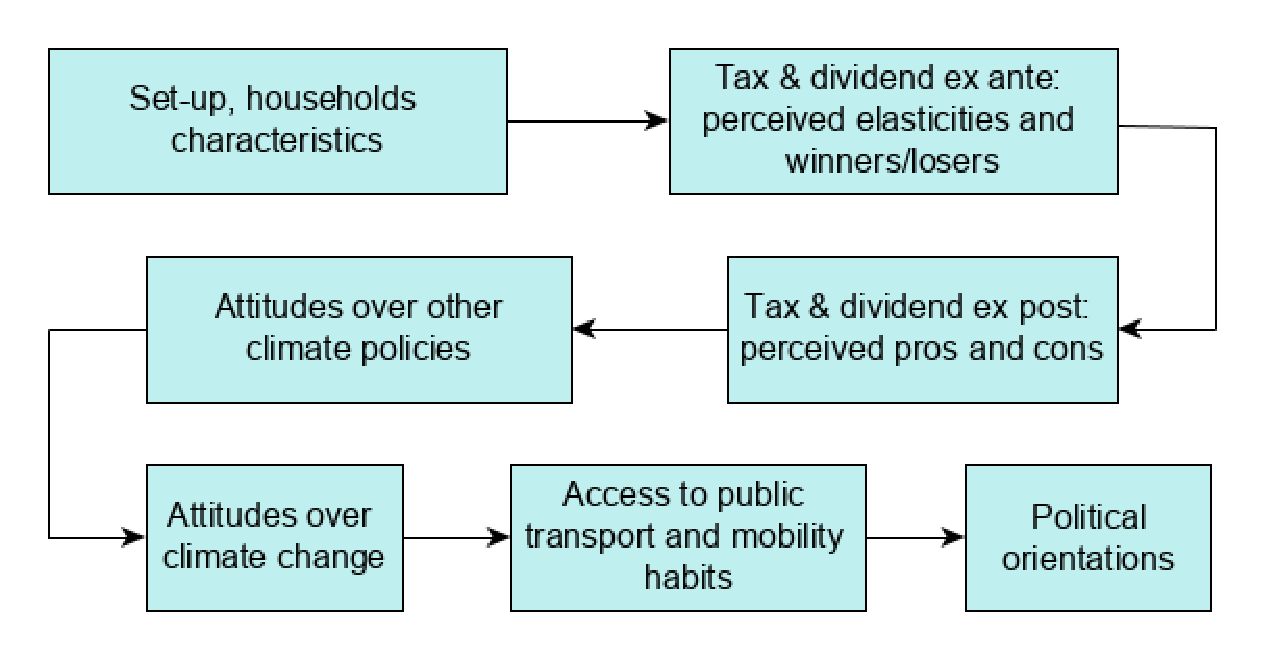
\includegraphics[width=\columnwidth]{Images_EPS/diagram_survey_attitudes.eps}
\caption{Diagram of the sequence of questions.}
\label{fig:survey}
\end{figure}
%
%
%
The survey starts by asking for households' socio-demographics and energy usage. The distribution of answers are much in-line with official statistics, as shown in Table \ref{tab:app-energetic-characs} in Appendix \ref{app:Raw-Data}. Then, we describe Tax \& Dividend reforms where the revenues of an increase in the French carbon tax by 50\euro{}/tCO$_\textnormal{2}$ are redistributed uniformly to all adults. We first allocate respondents randomly to a sectoral Tax \& Dividend reform, which concerns either gas and domestic fuel (i.e. housing energy), or gasoline and diesel (i.e. transportation energy). Respondents are asked to estimate their reaction to price changes, the reaction of French people, and how much purchasing power they would gain or lose from the policy. To this end, exact price variations and the amount transferred are provided, and respondents can choose among answers given in different brackets. Then, we study perceptions and support for a Tax \& Dividend on both sectors combined, before and after providing new information to the respondents. This new information is either that the policy is progressive, or whether their household would win or lose some purchasing power through the reform. Before providing information, we let respondents pick the categories of losers and winners from the reform; and after the information, they choose the benefits and the problems associated with this reform. We study these perceptions of the policy in the present paper, but please refer to our companion paper \citep{douenne_can_2019} for details and analyses on the other questions about Tax \& Dividend reforms. %

%

    \subsection{Eliciting attitudes} %


After inquiring about the support for Tax \& Dividend, we ask respondents to assess on a Likert scale different ways to recycle the revenues of a carbon tax. On another Likert scale, we examine opinions on other climate policies, notably new norms or Pigouvian taxes. We then measure respondents' knowledge about climate change by asking for its origin (anthropogenic or natural), its causes (in terms of gases and activities), which region it will most affect (between India and the European Union), and what reduction of emissions is needed by 2050 to respect the +2\textdegree{}C target. At the same time, we assess attitudes over climate change by asking respondents about the frequency with which they talk about it, the gravity of its consequences, the generations it will severely affect, and the entities responsible for its occurrence. We continue by surveying if and how climate change influences one's decision to have a child, under which conditions one would be ready to change their lifestyle to fight climate change, and whether one would be ready to adopt a sustainable lifestyle if policies were aligned to this goal. We also ask questions about diesel taxation. Then, we evaluate the respondents access to public transport, their mobility habits, and if there is room for changing these habits. Finally, we ask for their political preferences, including their positioning in relation to the Yellow Vests. The survey ends with a text box where the respondents can leave a comment.
%
%
%

\begin{figure}[b]
\centering
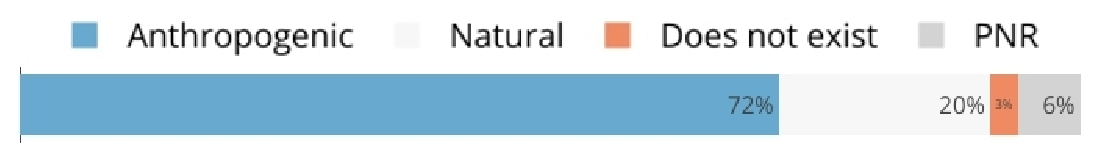
\includegraphics[width=\columnwidth]{Images_EPS/CC_cause_nolegend2.eps}
\caption{Perceived cause of climate change.}
\label{fig:cause}
\end{figure}

\begin{figure}[t]
\centering
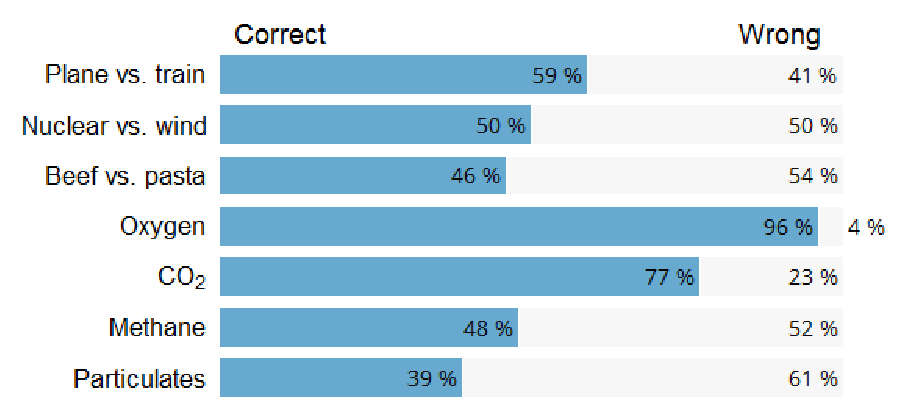
\includegraphics[width=\columnwidth]{Images_EPS/CC_knowledge_valbtr.eps}
\caption{Perceived factors of climate change.}
\label{fig:factors}
\end{figure}

\section{Attitudes over Climate Change\label{sec:attitudes_climate_change}}
    
To fully understand the root motivations to the support or rejection of climate policies, we first analyze the knowledge and perceptions over CC, as well as the reaction that people expect to address this phenomenon. As the paper focuses on explaining attitudes over policies, we relegate to online Appendix 1 some figures and some results from other surveys.
    
    \subsection{Knowledge\label{subsec:knowledge}}
%
As shown in Figure \ref{fig:cause}, knowledge that CC is anthropogenic is widespread (72\%) and the share who do not believe in climate change (CC) is marginal (4\%). The level of knowledge on the anthropogenic origin of CC is similar to that of other Western countries \citep{leiserowitz_international_2007,lee_predictors_2015,stokes_global_2015-1}: it is 66\% in the U.S. \href{https://news.gallup.com/poll/1615/environment.aspx}{(Gallup, 2019)} for example. At the same time, knowledge about climate science appears limited. Although 77\% of people correctly tick ``CO$_\textnormal{2}$'' as a greenhouse gas (GhG), Figure \ref{fig:factors} shows that almost as many people tick particulate matter (39\%) as methane (48\%). Admittedly, understanding the impacts of activities is more useful than erudition about chemical factors, but here again, knowledge is quite low. We assess such awareness using pairs of comparable activities whose GhG footprint differ by a factor 20 (beef steak vs. pasta, plane vs. train) or whose footprint are similar (nuclear vs. wind power).\footnote{Appendix \ref{app:footprint} details how the figures were obtained.} We ask whether it is true that one activity emits 20 times more GhG than the other, as a way to express precisely that one is ``much more'' polluting than the other. For each pair, around half of the sample is correct. The bulk of respondents pick two correct answers out of three (44\%), but more get them all wrong (19\%) than all right (15\%). 

Not only do most people fail to fully understand the factors and consequences of CC, but they also fail to grasp the degree of reaction needed to tackle it. When informed that ``each French person emits on average the equivalent of 10 tons of CO$_\textnormal{2}$ per year'' and asked what the figure should be in 2050 to ``hope to contain global warming to +2\textdegree{}C in 2100 (if all countries did the same)'', 59\% answer 5 or more (see Figure \ref{fig:target_emission}). Only 17\% select a correct answer: 0, 1 or 2 (see Appendix \ref{app:sources} for why these are correct).

\begin{figure}[t]
\centering
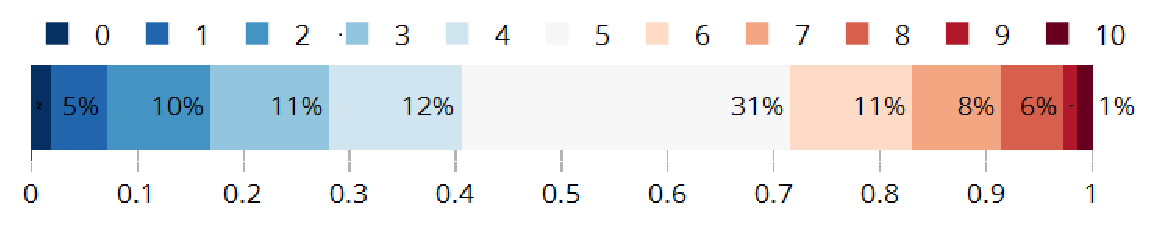
\includegraphics[width=\columnwidth]{Images_EPS/CC_target_emission_nolegend.eps}
\caption{Perceived GhG emission p.c. required in 2050 to limit global warming to +2\textdegree{}C (in tCO$_\textnormal{2}$eq/yr), given that it is now 10.}
\label{fig:target_emission}
\end{figure}

%


\begin{figure}[!htbp]
\centering
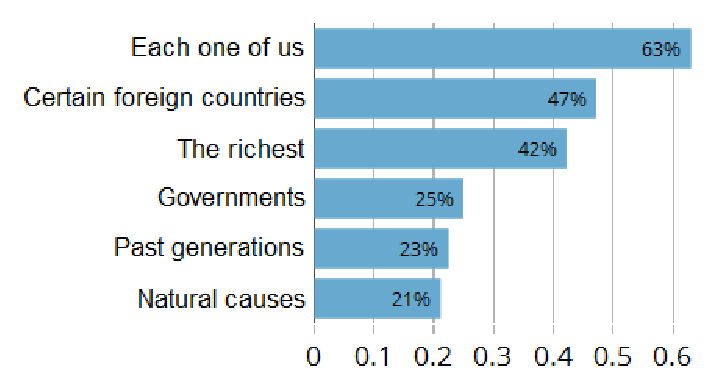
\includegraphics[width=0.75\columnwidth]{Images_EPS/CC_responsiblec.eps}
\caption{Entities perceived responsible for climate change.}
\label{fig:responsible}
\end{figure}

\begin{figure}[t]
\centering
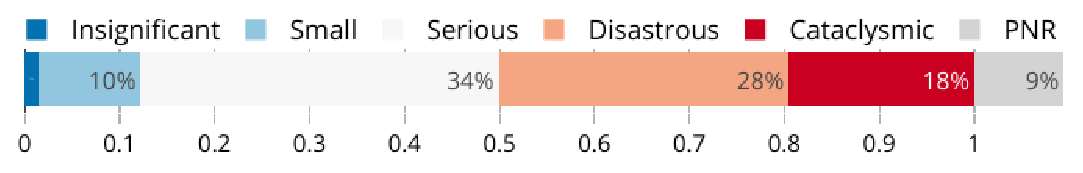
\includegraphics[width=\columnwidth]{Images_EPS/CC_effects_nolegend.eps}
\caption{Perceived gravity of climate change.}
\label{fig:gravity}
\end{figure}

\citet{millner_beliefs_2016} propose several mechanisms to explain people's lack of understanding about climate change: in addition to the difficulty of grasping gradual changes, they emphasize the complexity of drawing a causal link between diffuse causes and distant consequences.\footnote{Actually, even MIT students struggle with this \citep{sterman_risk_2008}.} Failing to assimilate the underlying channels may blur the link between people's own behavior and consequences for the climate. Thus, we can wonder if people understand who would have to make the mitigation effort in a sustainable scenario, i.e. who is responsible for CC.


    \subsection{Perceptions\label{subsec:opinions}}
    %
%
As shown in Figure \ref{fig:responsible}, 63\% acknowledge that ``each one of us'' is responsible for CC, and less people ascribe the responsibility to ``certain foreign countries'' (47\%), ``the richest'' (42\%), or any other agent.  Not only do people seem lucid concerning the agents causing CC, but a vast majority also foresees worrying consequences if humanity does nothing to limit it. Figure \ref{fig:gravity} shows that 19\% see the impacts as ``cataclysmic, humankind would disappear'', 18\% as ``disastrous, lifestyles would be largely altered'', 28\% as ``grave, because there would be more natural disasters'', while only 11\% think damages would be ``small, because humans would be able to live with it'' or ``insignificant, or even beneficial''. 

%

%

Overall, these results indicate that most people understand the fundamentals of climate issues, including the root causes and the scale of the problem, but that only a minority has thought of CC deeply enough to comprehend its factors and the pathways to tackle it.
%

%
%
    
%
%

\begin{figure}[t]
\centering
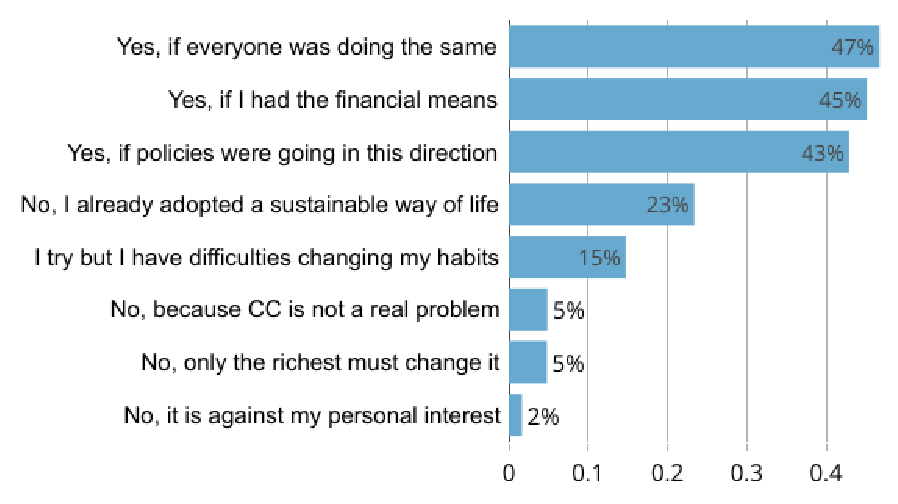
\includegraphics[width=\columnwidth]{Images_EPS/change_if_no.eps}
\caption{Respondent could change their lifestyle under a condition.}
\label{fig:condition}
\end{figure}

    \subsection{The Reaction Needed\label{subsec:reaction}}

Given that many people may not realize the extent of the transition needed to reach sustainability, and that others may be discouraged precisely by the sheer magnitude of such a transition, we can wonder how willing people are to contribute to its success. An encouraging finding for the transition is that 65\% are ``willing to adopt an ecological lifestyle (i.e. eat little red meat and make sure to use almost no gasoline, diesel nor kerosene)'', assuming that ``all states in the world agree to firmly fight climate change, notably through a transition to renewable energy, by making the richest contribute, and imagining that France would expand the supply of non-polluting transport very widely'', while only 17\% answer ``No'' (the others do not take a side). While the phrasing removes most grounds against a change in lifestyle, we inquire under which conditions people would be willing to adopt such a change (see Figure \ref{fig:condition}). 82\% of respondents would be willing to change their lifestyle under at least one of the three conditions proposed: sufficient financial resources, an alignment of policies to this goal, or an adjustment of others' behavior (about 45\% each).
%

%

Finally, a substantial fraction of people incorporates ecological constraints in their life choices. Indeed, 15\% call themselves ecologist (the most picked political identity outside of the left-right spectrum, see Appendix \ref{app:stats_des}), 23\% claim they already adopted a sustainable way of life, and 20\% say the CC ``has had or will have an influence in their decision to have a child''. 

%

%
%
%
%


\section{Attitudes over Carbon Tax and Dividend} \label{sec:attitudes_carbon_tax}

%

%

%
Most French people are aware and concerned about climate change and claim to be willing to exert efforts to fight it. Yet, the government's attempt to introduce a carbon tax to deal with French emissions resulted in a widespread popular protest. To understand this paradox, we investigate the preferences over a Tax \& Dividend policy: an increase of 50\euro{}/tCO$_2$ in the current French carbon tax, with a uniform lump-sum redistribution of the additional revenue to all adults. This policy differs from the official one whose revenue was mostly used to fund the general budget. Respondents are given the associated increase in energy prices so that the direct costs are salient: $+13\%$ (resp. $+15\%$) for gas (resp. domestic fuel), and $+0.11$\euro{} (resp. $+0.13$\euro{}) for a liter of gasoline (resp. diesel). They are also told that the transfer would amount to 110\euro{} per adult annually. %

    \subsection{Widespread rejection}

%
French people would largely reject the proposed policy. Only 10\% of our respondents declare they would approve it, while 70\% say they would not (see Figure \ref{fig:approval}). As shown in our companion paper \citep{douenne_can_2019}, this rejection can be explained by erroneous perceptions about the policy's outcome, such as an overestimation of its impact on one's purchasing power. For instance, 30\% of people who use neither gas nor domestic fuel believe their household would lose from an equally redistributed increase in taxes on these goods. Interestingly, the salience of costs appears critical in people's answer. At a later stage of the survey, we ask respondents whether they would agree to increase the carbon tax if the revenue was returned to all households, without mentioning the impact on prices. The question is asked along with a package of other environmental policies (see section \ref{sec:attitudes_other_policies}). In this case --- where the benefits are more salient than the costs --- we find a much higher approval rate of 37\%. Another survey conducted in March 2019 (\href{https://drive.google.com/file/d/1ne1nUsJJqY1PYFOs9dH9uK6mLw39R1QY/view}{OpinionWay, 2019}) assesses acceptance for a \uline{reintroduction} of the carbon tax increase in 2021. They find intermediary results with an approval rate of 21\%. %

%

\begin{figure}[t]
\centering
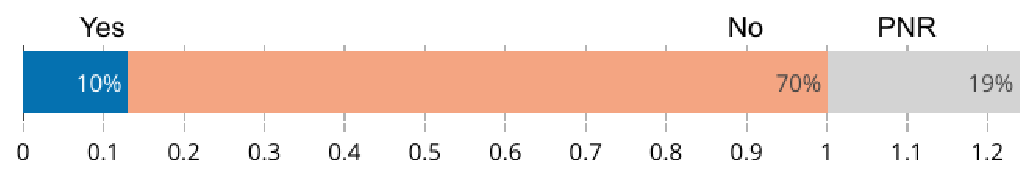
\includegraphics[width=\columnwidth]{Images_EPS/approval_trim.eps}
\caption{Approval of Tax \& Dividend.}
\label{fig:approval}
\end{figure}
%

%

The low level of acceptance observed partly results from recent events. In July 2018, \citet{ademe_representations_2018} found that 48\% of French people thought it was desirable to increase the carbon tax, a figure similar to those of other countries \citep{brechin_public_2010}. The discrepancy between 2018 and 2019 can be explained by the ``campaign effect'' highlighted by \citet{anderson_can_2019}: support for a carbon tax decreases substantially after it enters the public debate. Indeed, the French carbon tax was brought under the spotlight in the end of 2018, after high oil prices triggered the Yellow Vests movement.
%
%
%

%

%

%
%

%
%
%

    \subsection{Perceived winners and losers}

Figure \ref{fig:winners_losers} represents the share of respondents who expect different household categories to win or lose from the policy. Income appears to be the most critical divide, with a non-monotonic relationship. 30\% of respondents expect the richest to win while only 2\% think they would lose. On the contrary, 40\% more people think that the poorest would lose rather than win, a difference even higher for the middle class --- the category most expected to lose --- at 53\%. To half of respondents, we framed the question about winners and losers specifically in terms of ``purchasing power''. The objective was to see if some categories were commonly seen as losing in welfare although they could gain in monetary terms, or conversely. The results look very much alike for both formulations, except that the shares of people expecting poorer households to gain (5.8\%) and richer households to lose (0.9\%) are significantly larger when asked in terms of purchasing power: 10.2\% and 2.1\%, respectively (see online Appendix 2). Overall, respondents perceive the Tax \& Dividend as regressive. As shown by a large body of literature \citep[e.g.][]{west_williams_04,bento_distributional_2009,williams_initial_2015}, and more specifically in our companion paper \citep{douenne_can_2019}, these beliefs are at odds with the true distributive effects of this proposed policy. %
%
\begin{figure}[t]
\centering
\begin{subfigure}[b]{\columnwidth}
   \caption{Winners}
   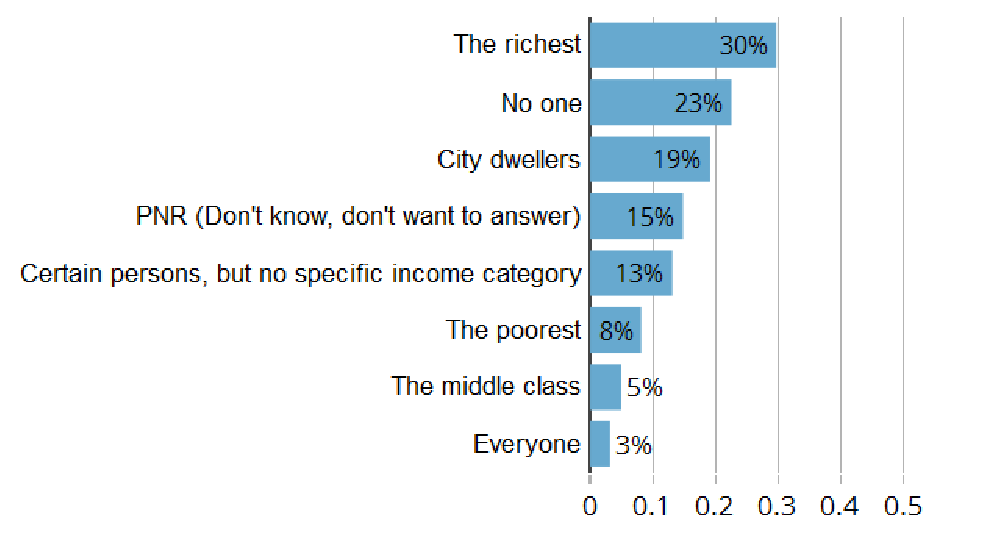
\includegraphics[width=\columnwidth]{Images_EPS/tax_winners_synchro.eps}
\end{subfigure}

\begin{subfigure}[b]{\columnwidth}
\vspace{0.3cm}
   \caption{Losers}
   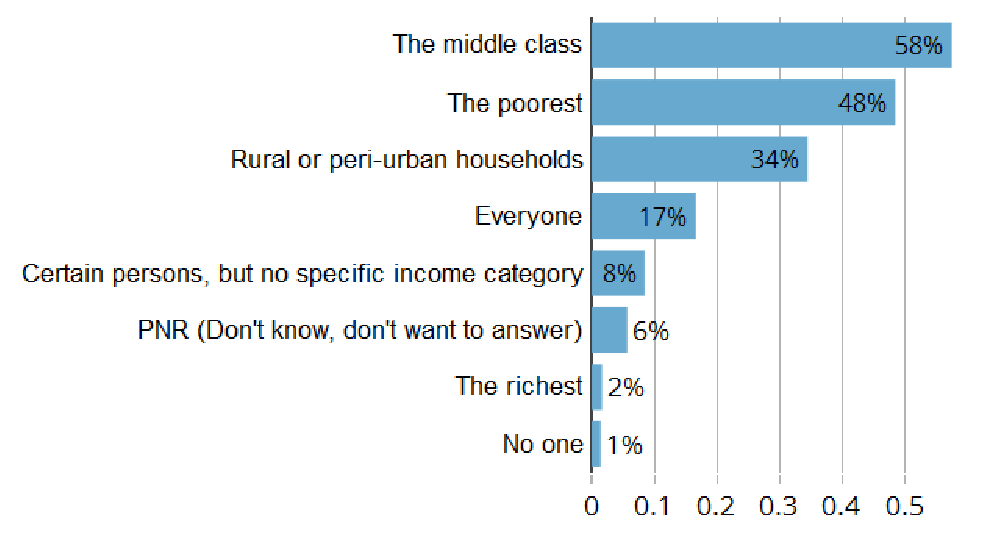
\includegraphics[width=\columnwidth]{Images_EPS/tax_losers_synchro.eps}
\end{subfigure}
\caption{Perceived winners and losers from Tax \& Dividend}
\label{fig:winners_losers}
\end{figure}

Beyond the income dimension, people tend to identify city dwellers as potential winners from the Tax \& Dividend (third position at 19\%), while rural and peri-urban households are rather expected to lose (third position at 34\%). We also see that people report on average more categories for expected losers than winners: 1.74 vs. 1.16. The high ranks of ``no one'' for winners (second) and of ``everyone'' for losers (fourth) further suggest that respondents do not see our policy as a zero-sum game. %
%
    \subsection{Perceived pros and cons}

%

%

Previous studies have highlighted that distributive effects are a critical determinant of carbon tax acceptance \citep[e.g.][]{kallbekken_saelen_2011,brannlund_tax_2012,gevrek_public_2015}. When asked about the problems associated with the Tax \& Dividend, the main response is that the tax would penalize rural households (47\%). Interestingly, this concern comes before the threat that the tax could penalize the poorest (sixth position with 29\%), although more people report the poorest as a category of people expected to lose. The second and third concerns are that the policy is simply a pretext to increase taxes (43\%) --- a worry documented by \citet{dresner_social_2006} and \citet{klok_et_al_2006} --- and that it would be ineffective to reduce pollution (37\%). Related to this last point is the perceived lack of alternatives, seen as insufficient or too expensive (31\%). This problem has been previously stressed by \citet{kallbekken_aasen_2010} in a focus group study: people do not see the point of taxing fossil fuels if they cannot substitute for other technologies. This last reason is stated as frequently as concerns over the impact on one's own purchasing power (fourth with 31\%). As shown in \citet{douenne_can_2019}, self-interest largely affects acceptance of the Tax \& Dividend, but this concern could sound too egoistic when stated in a direct way. While previous studies have pointed out concerns over the negative impact of carbon taxation on the economy \citep[e.g.][]{thalmann_public_2004,carattini_green_2017}, this problem comes last (14\%) and does not seem to represent an important obstacle for public support in the current context. %

%

\begin{figure}[t]
\centering
\begin{subfigure}[b]{\columnwidth}
   \caption{Benefits}
   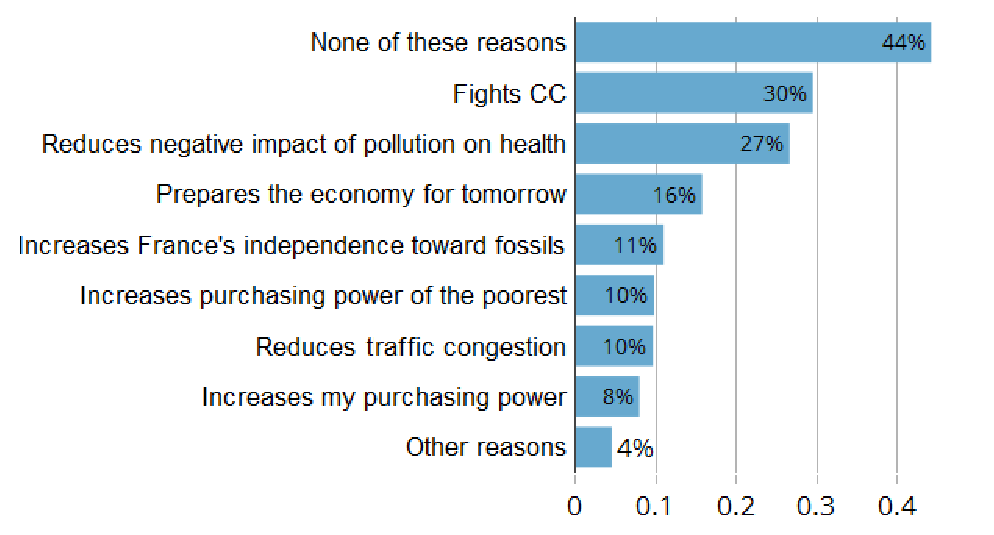
\includegraphics[width=\columnwidth]{Images_EPS/CC_benefits_synchro.eps}
\end{subfigure}

\begin{subfigure}[b]{\columnwidth}
\vspace{0.3cm}
   \caption{Problems}
   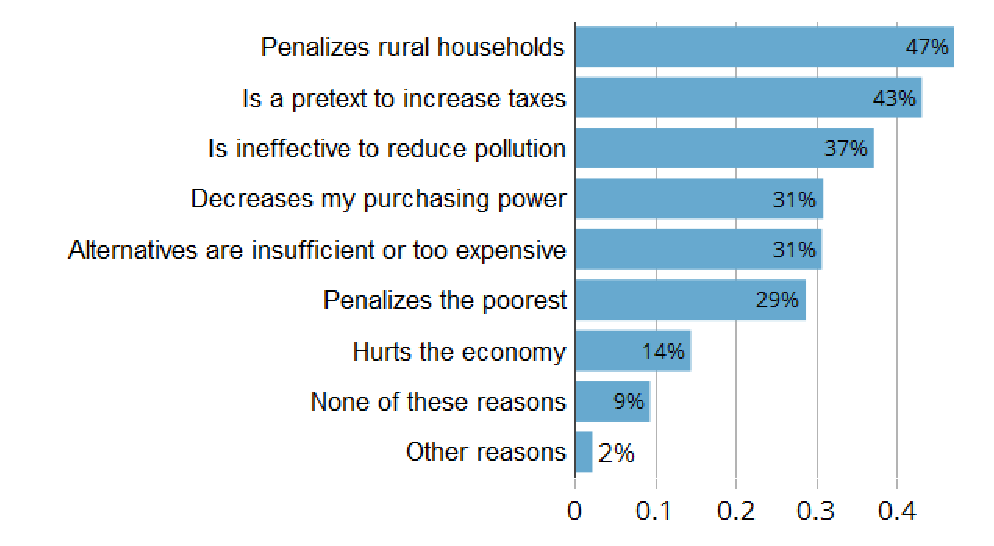
\includegraphics[width=\columnwidth]{Images_EPS/CC_problems_synchro.eps}
\end{subfigure}
\caption{Perceived benefits and problems from Tax \& Dividend}
   \label{fig:benefits_problems}
\end{figure}

Respondents are suggested to pick at most three answers among both problems and benefits. On average, respondents pick 2.36 problems --- and 53\% pick at least 3 --- against 1.14 benefits, excluding the most popular: ``None of these reasons'' (44\%). This option comes far ahead of the second and third, ``fight climate change'' (30\%) and ``reduces negative impact of pollution on health'' (27\%). Still, environmental benefits are much more cited than economic ones. This result is likely due to people's pessimism about the outcome of the policy, but it might also reflect the limited importance given to economic consequences of the carbon tax, as already suggested by problems commonly cited. %
%

    \subsection{Consumption and mobility constraints}

The perceived problems identified above suggest a rationale for people's opposition towards carbon taxation: if people think the tax is ineffective, because their consumption is constrained and affordable alternatives are lacking, then taxing carbon can be perceived as a pretext to increase taxes. %

    \subsubsection{Perceived elasticities}

In order to understand to what extent people feel constrained with respect to their energy consumption, we elicit their subjective price elasticity for transport and domestic energies. We adopt the phrasing of \citet{baranzini_effectiveness_2017} and ask the expected decrease in energy consumption that would follow an increase in prices. To avoid dealing with small percentages, which people usually find more difficult to compare, we ask for the reaction to a 30\% increase in the price of heating (or equivalently, an increase of 0.50\euro{} per liter in fuel prices). Although sufficiently high to foster a significant response on demand, these changes are realistic in the medium run, and should not lead people to report long-term elasticities. Respondents may select their answer among 5 brackets. They are asked to estimate their own reaction as well as that of French people. Figure \ref{fig:elasticities_agg} presents the results.

%

\begin{figure}[t]
\centering
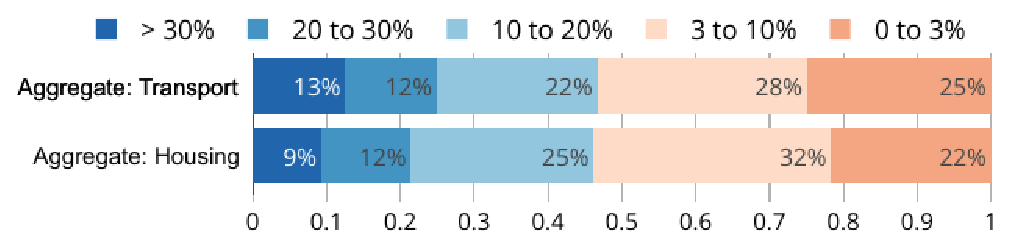
\includegraphics[width=\columnwidth]{Images_EPS/elasticities_agg_valb.eps}

\includegraphics[height=0.3cm]{Images_EPS/blank.eps}
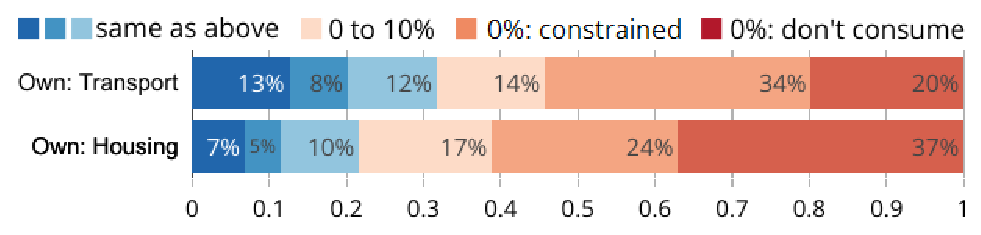
\includegraphics[width=\columnwidth]{Images_EPS/elasticities_perso_valbuena.eps}
\caption{Perceived aggregate and own elasticities.}
\label{fig:elasticities_agg}
\end{figure}

\begin{figure}[b]
\centering
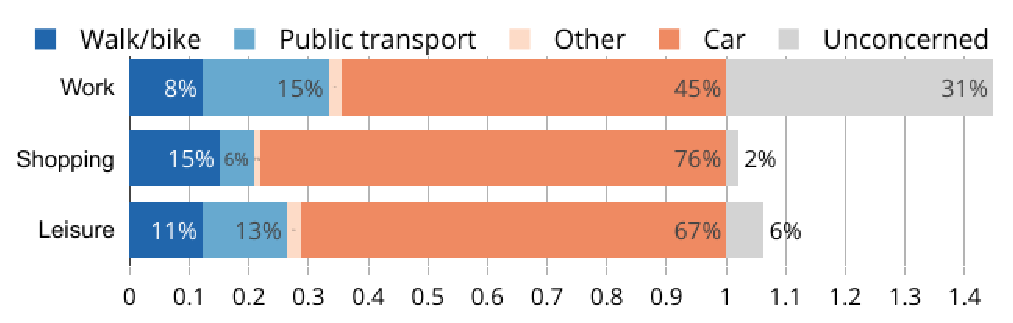
\includegraphics[width=\columnwidth]{Images_EPS/transports_use_trim.eps}
\caption{Mode of transportation by activity.}
\label{fig:transports_use}
\end{figure}

%
54\% (resp. 61\%) of respondents consider that such an increase in prices would not lead them to reduce their transport (resp. domestic) energy consumption. This expected inelastic behavior is mainly due to mobility constraints for transport (64\% of cases) while it mostly reflects a non-fossil heating type for housing (61\%). Excluding people reporting inelastic behavior because of insignificant initial consumption, about 40\% of people feel constrained and expect to not lower their consumption following price increases. Still, respondents perceive transport fuel price elasticity of French people at $-0.45$ on average, and their own elasticity at a consistent $-0.36$ (after re-weighting by fuel expenditures). Concerning housing energy, aggregate and personal subjective elasticities are respectively $-0.43$ and $-0.33$. Overall, these subjective elasticities compare well to the ones found in the literature for French households, although they are slightly over-estimated (in absolute value) for housing.\footnote{For transports, estimates from the literature lie around $-$0.4 \citep{clerc_marcus,bureau_distributional_2011,douenne_vertical_2018}. For housing, the values are lower, typically around $-$0.2 \citep{douenne_vertical_2018,clerc_marcus}.}

%

%

%

%

%

\begin{figure}[t]
\centering
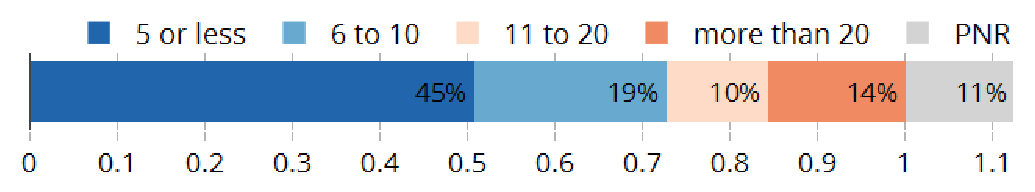
\includegraphics[width=\columnwidth]{Images_EPS/transports_distance_trim.eps}
\caption{Walking distance to the nearest stop, in minutes.}
\label{fig:transports_distance}
\end{figure}

\begin{figure}[t]
\centering
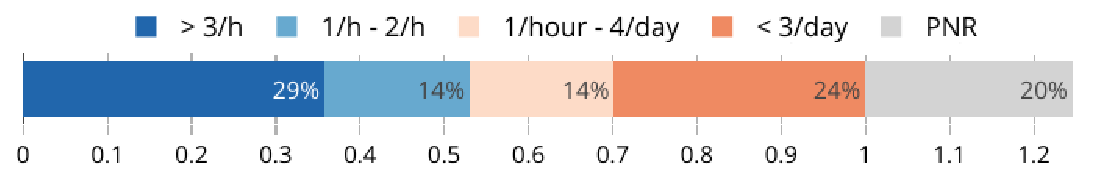
\includegraphics[width=\columnwidth]{Images_EPS/transports_frequency_trim.eps}
\caption{Frequency of public transport at the nearest stop.}
\label{fig:transports_frequency}
\end{figure}

\begin{figure}[b]
\centering
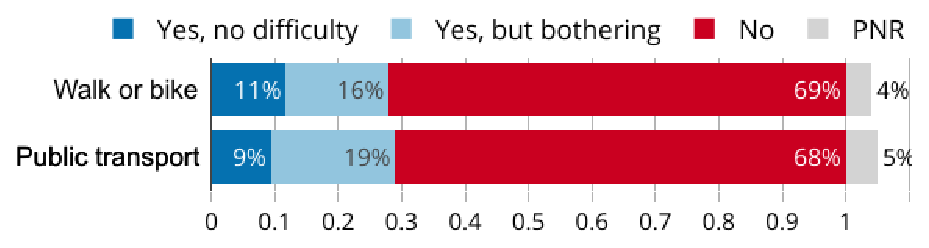
\includegraphics[width=\columnwidth]{Images_EPS/transports_work.eps}
\caption{Among those who commute to work by car, possibility to change the transportation mode, depending on the alternative.}
\label{fig:transports_work}
\end{figure}
    
\begin{figure}[b]
\centering
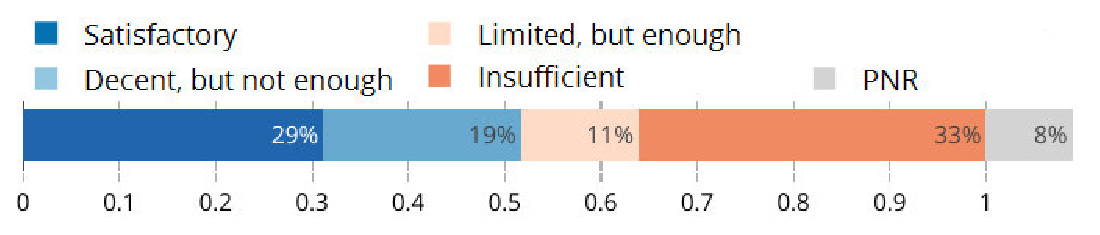
\includegraphics[width=\columnwidth]{Images_EPS/transports_opinion_trim.eps}
\caption{Supply of public transport where the respondent lives.}
\label{fig:transports_opinion}
\end{figure}

    \subsubsection{Mobility and public transport}
    %

To assess the level of dependence on automobiles, which we include as a determinant for preferences in Section \ref{sec:determinants}, we study mobility habits and access to public transport. Figure \ref{fig:transports_use} indicates that 65\% of employed people drive to work, and that car usage is even more common for grocery shopping or leisure activities. This figure is confirmed by the national transport survey \href{http://www.progedo-adisp.fr/enquetes/XML/lil-0634.xml}{ENTD (2008)} conducted by Insee and analyzed in \cite{pappalardo_mobilite_2010}, which reveals that a majority still uses a car for trips of 1 to 2 km. Even though 73\% live within a 10 minute walk to a public transit stop (Figure \ref{fig:transports_distance}), coverage and frequency of public transport is often too low (Figure \ref{fig:transports_frequency}) to compete with the speed, comfort, and flexibility of automobiles. Indeed, 58\% of those who commute by car declare that they could neither substitute it with public transport nor walking or cycling, and only 15\% could use one of these alternative without major difficulties (Figure \ref{fig:transports_work}). Further evidence indicates that the lack of alternatives is a main factor for car usage, besides apparent taste for a vehicle that remains a symbol of freedom. Figure \ref{fig:transports_opinion} shows that 52\% of respondents state that supply of public transport where they live is ``insufficient'' or ``decent, but should be increased'', while 40\% find it ``satisfactory'' or ``limited, but sufficient''. From this perspective, ``green public investments and carbon taxes appear to be complementary, and in the timing of climate policy it would be justified to carry out the former before implementing the latter'', as \cite{bureau_pour_2019} suggest. Alongside an increase in the supply of alternatives, climate policies could also address the demand for mobility, e.g. by revitalizing town centers and limiting urban sprawl.

%

%

%
%
%

%

\section{Attitudes over Other Policies}\label{sec:attitudes_other_policies}

The previous section has shown that our Tax \& Dividend was largely rejected by French people. As climate policies are urgently needed, it appears necessary to assess whether other designs and instruments would be met with a higher support. This section first examines public opinion about several alternative uses for the carbon tax revenue and then turns to other environmental and climate policies.

    \subsection{Preferred Revenue Recycling}

%
We asked respondents to what extent they would accept an increase in the carbon tax for different uses of the revenue. As the exact cost of the tax was not specified, the benefits of the revenue recycling were made relatively more salient, which explains higher acceptance rates compared to our Tax \& Dividend. Still, this question enables to compare answers relative to one another.

        \subsubsection{Investments in energy transition}

%
%
%
Figure \ref{fig:recycling} reports people's responses to each proposed scenario. Overall, the preferred revenue recyclings are investments in the energy transition. This result is consistent with various papers showing that earmarking the revenue of the tax for environmental purposes largely increases public support \citep[for a review of the literature, see for instance][]{kallbekken_aasen_2010,carattini_overcoming_2018}. As people tend to see carbon taxation as effective only if it finances green investments \citep{saelen_kallbekken_2011}, these policies legitimize the implementation of a tax and increase its acceptance. In addition, the large approval for a policy investing in non-polluting transport can be explained by people's desire for mobility alternatives, the lack of which was identified as an important problem with our Tax \& Dividend (see section \ref{sec:attitudes_carbon_tax}). %

%

%

\begin{figure}[!htbp]
\centering
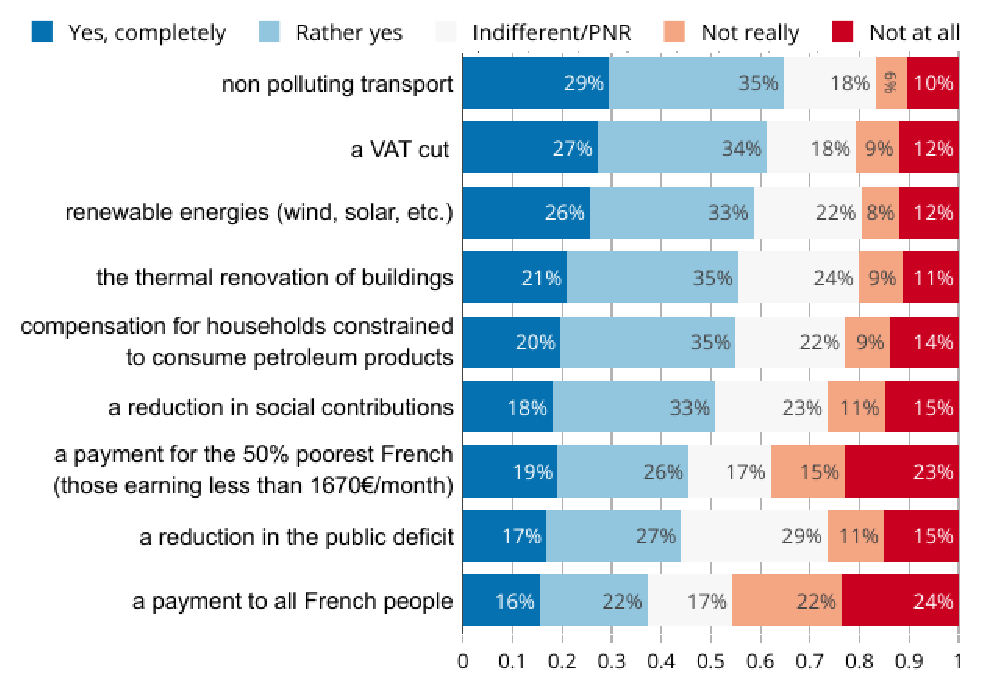
\includegraphics[width=\columnwidth]{Images_EPS/tax_condition_valc.eps}
\caption{Approval of a carbon tax if its revenue finances...}
\label{fig:recycling}
\end{figure}

        \subsubsection{Transfers to households}
%
While previous literature has shown that distributive concerns matter for carbon tax approval, the common tool proposed by economists to address this issue --- lump-sum transfers --- is not met with resounding support. Out of the nine proposed mechanisms, the standard flat recycling comes last (with 37\% approval), and a transfer targeted to the bottom 50\% comes seventh (46\%). Consistent with our previous finding that people are concerned that the carbon tax may penalize rural and peri-urban households, the preferred ``lump-sum'' transfer is the one targeted to people constrained with respect to their consumption of petroleum products (fifth with 55\% approval). These results echo the findings of \citet{kallbekken_et_al_2011} who showed that people tend to prefer more narrowly targeted revenue recycling, possibly because of distributional concerns. %

The relatively low support for compensation mechanisms should however not be understood as a lack of concern about purchasing power or distributive effects. As shown in section \ref{sec:attitudes_carbon_tax}, the distributive properties of lump-sum transfers are not well understood. Perhaps surprisingly, the second preferred mechanism for revenue recycling is a reduction in the VAT rate (61\% approval). The main rationales for this support are the benefits to one's purchasing power and the perceived distributive effects. As the VAT is known to be a regressive tax, people may perceive it fair to compensate an increase in the regressive carbon tax with a decrease in the VAT. Although such a mechanism would be less favorable to poorer households --- who spend less in VAT in absolute value, and would therefore receive less than from a uniform transfer --- it may not be perceived as such. %

%

        \subsubsection{Double dividend and public deficit}

The last two options propose to use the carbon tax revenue to reduce social contributions, or the public deficit. These mechanisms come respectively in sixth and eighth position with 51\% and 44\% of approval. These results can be linked to the low level of concern regarding the impact of a carbon tax on the economy documented in section \ref{sec:attitudes_carbon_tax}. They are also consistent with previous focus group studies \citep[e.g.][]{kallbekken_aasen_2010}, including in France where \citet{deroubaix_rise_2006} found that people did not understand why the revenue of an environmental tax reform should be used to tackle unemployment.


\begin{figure}[t]
\centering
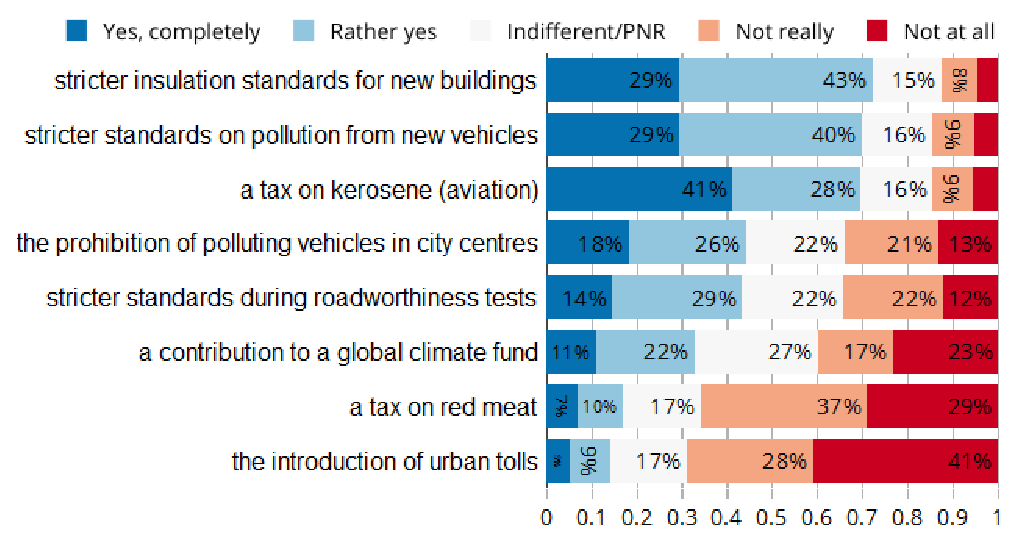
\includegraphics[width=\columnwidth]{Images_EPS/environmental_policies.eps}
\caption{Approval of different climate policies.}
\label{fig:policies}
\end{figure}

    \subsection{Other Instruments}

%

%
Under a binding acceptability constraint, alternative instruments become relevant, even if Pigouvian taxes may be more cost-effective \citep[e.g.][]{goulder_parry_2008}. To elicit people's preferred environmental policies, we ask respondents whether they would support eight different propositions. To make these questions easier to answer, the exact mechanisms and their associated costs and benefits are unspecified. The answers reported should therefore be taken cautiously as people could change their mind once faced with clear trade-offs. Still, this exercise is informative about people's first reactions to different proposals.

%

%

%
%
%
%
%
%

        \subsubsection{Other Pigouvian taxes}

%
%
%
Figure \ref{fig:policies} shows that among the eight options, the most strongly supported is a tax on kerosene (70\% of ``Yes'' including 41\% of ``Yes, completely''). The main rationale could be a broadly perceived effectiveness of the tax if people view aviation as an important source of emissions, and the distributive effect of such policy since richer people fly more.\footnote{In France in 2008, people in the top income decile travelled by plane about seven times more than the bottom 50\% of the income distribution \citep{pappalardo_mobilite_2010}. Furthermore, kerosene's emissions are taxed only through the EU-ETS, hence at a far lower rate than diesel and gasoline. This discrepancy has been highlighted in the public debate.} In sharp contrast, only 17\% of our survey respondents approve a tax on red meat, a policy ranked second-to-last. One could explain this lower acceptance rate by the belief that such policy would be ineffective, as we have shown in section \ref{sec:attitudes_climate_change} that less than half of respondents know that beef has a high carbon footprint. Additional reasons for its rejection could be the perceived negative impact on purchasing power, and the feeling that the policy is too coercive and targets a behavior difficult to change \citep{de_groot_schuitema_2012}. Overall, this evidence confirms that people are not opposed to Pigouvian taxes \uline{per se}, and that acceptance varies significantly depending on the target and the perceived outcome of the instrument.

%

%

        \subsubsection{Norms}

Among all proposed instruments, the two most approved are norms. 72\% and 70\% of respondents declared being in favor of stricter standards for the insulation of new buildings and for the pollution of new vehicles, respectively. It is unclear to what extent people are aware of the ``hidden costs'' of such policies. For instance, fuel economy standards in the US have been estimated to be three to six times more costly than a tax on gasoline for similar abatement levels \citep{jacobsen_2013}, and as possibly more regressive \citep{jacobsen_2013, davis_knittel_2019, levinson_2019}. The exact properties of these instruments are of course specific to their design, but it is likely that their popularity partly reflects the underestimation of their costs.

For urban transport policies as well, standards are preferred to price instruments. While the prohibition of polluting vehicles in city centers comes fourth on the list of preferred options with 44\% approval, the introduction of urban tolls comes last with only 14\%. In a survey on urban road pricing, \citet{jones_1998} identifies the main deterrent for these mechanisms. While some are specific to congestion charges, the other perceived problems are very much alike those identified for our Tax \& Dividend: ineffectiveness, unfairness and the feeling that it is just another tax.

        \subsubsection{Diesel taxation}

%

\begin{figure}[b]
\centering
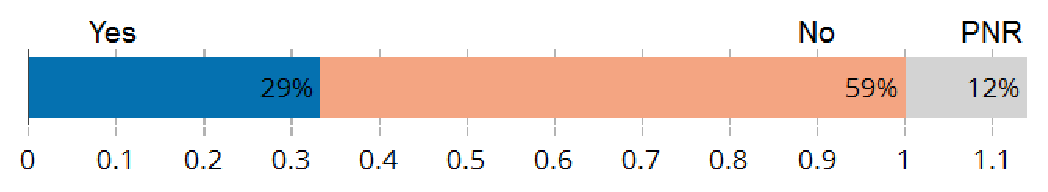
\includegraphics[width=0.9\columnwidth]{Images_EPS/diesel_catch_up_trim.eps}
\caption{Approval of a catching-up of the diesel tax.}
\label{fig:diesel}
\end{figure}

The strong opposition of the Yellow Vests against energy taxes did not only lead the government to reverse the planned carbon tax trajectory. The additional tax increases initially scheduled for diesel --- to catch-up with the currently higher rates imposed on gasoline despite diesel's high social cost from air pollution  --- have also been abandoned.\footnote{Three increases of +0.026\euro{}/L were initially scheduled for January 2019, 2020 and 2021.}  In our survey, we ask respondents whether they would therefore accept an increase in diesel tax to catch up with that of gasoline. As illustrated by Figure \ref{fig:diesel}, 59\% of respondents answer they would not, while 29\% say they would (12\% ``PNR''). Among the 57\% of households who own a diesel vehicle, the opposition augments to 80\%. The geographic difference is also striking as 73\% of rural households would be opposed, vs. only 40\% of those living in the Paris agglomeration. As shown in our online Appendix 3.1, these two determinants appear as the most important divides with respect to diesel taxation.
%

%

%

%


%
%

%

%
%
%
%
%
%


%

\section{Determinants of Attitudes\label{sec:determinants}}

To understand what factors foster environmentally-friendly attitudes, we explore the socio-demographic determinants of attitudes over CC, the correlations between knowledge and perception of CC, and how these attitudes over CC as well as socio-demographics shape preferences for policies. 

    \subsection{Attitudes over climate change}\label{sec:determinants_attitudes_CC}

%
Table \ref{tab:determinants_attitudes_CC} shows the main socio-demographic determinants of different attitudes towards CC: the knowledge that CC is anthropogenic (columns 1-3), an index of knowledge about CC (4) and the perception that CC is ``disastrous'' or ``cataclysmic'' (5-6). To build the index of knowledge, we aggregate different variables corresponding to the different kinds of knowledge about CC identified by \citet{kiel_einfuhrung_2002} \citep[see also][for a summary]{hoppe_what_2018}. 

We first compute a score for the question asking the emission target p.c. required to limit CC (see section \ref{subsec:knowledge}). Denoting $t$ as the respondent's answer (from 0 to 10 tCO$_2$/yr), we define the score as:

\begin{equation}
\textnormal{score emission target}=\begin{cases}
3 & \text{if }t\leq2\\
2 & \text{if }t\in\left[3;4\right]\\
1 & \text{if }t\in\left[5;6\right]\\
0 & \text{if }t\geq7
\end{cases}
\end{equation}

\noindent and we then aggregate this score with other answers:

\begin{align}
\textnormal{knowledge} = & \; 3\cdot \textnormal{CC anthropogenic}-2\cdot \textnormal{CC doesn't exist} \nonumber \\ & + \textnormal{ score factors}+\textnormal{score emission target} \label{eq:knowledge2}
\end{align}

where ``score factors'' is the sum of correct answers to factors of CC (see Figure \ref{fig:factors}), and the two first variables in the formula are dummies. The relative weights of the variables correspond to the loadings of a one-factor analysis, ensuring that our index captures the most determinant elements of knowledge.\footnote{See online Appendix 4 for more details.} The original index ranges from $-$2 (no respondent) to +13 (22 respondents), and has quartiles of 6, 8 and 9. In the regressions, we normalize this index by subtracting the mean (7.6) and dividing by the standard deviation (2.5). Finally, we run OLS regressions of the three attitudes over CC on various socio-demographics, household characteristics, and political orientation. We report only the most relevant variables, but describe the entire list of covariates in Appendix \ref{app:covariates}. We confirm that logistic regressions yield similar results (see online Appendix 5).


\begin{table*}[!htbp] \centering 
  \caption{Determinants of attitudes towards climate change (CC).} 
  \label{tab:determinants_attitudes_CC} 
\makebox[\textwidth][c]{ \begin{tabular}{@{\extracolsep{5pt}}lcccccc} 
\\[-1.8ex]\hline 
\hline \\[-1.8ex] 
\\[-1.8ex] & \multicolumn{3}{c}{CC is anthropogenic} & Knowledge about CC & \multicolumn{2}{c}{CC is disastrous} \\ 
\\[-1.8ex] & (1) & (2) & (3) & (4) & (5) & (6)\\ 
\hline \\[-1.8ex] 
 Interest in politics (0 to 2) & 0.032$^{**}$ &  &  & 0.137$^{***}$ & 0.051$^{***}$ &  \\ 
  & (0.013) &  &  & (0.028) & (0.014) &  \\ 
  Ecologist & 0.135$^{***}$ &  &  & 0.404$^{***}$ & 0.192$^{***}$ &  \\ 
  & (0.024) &  &  & (0.053) & (0.027) &  \\ 
  Yellow Vests: PNR & $-$0.098$^{***}$ &  &  & $-$0.142$^{**}$ & $-$0.093$^{***}$ &  \\ 
  & (0.033) &  &  & (0.071) & (0.036) &  \\ 
  Yellow Vests: understands & $-$0.038$^{*}$ &  &  & $-$0.100$^{**}$ & $-$0.051$^{**}$ &  \\ 
  & (0.022) &  &  & (0.048) & (0.024) &  \\ 
  Yellow Vests: supports & $-$0.098$^{***}$ &  &  & $-$0.223$^{***}$ & $-$0.061$^{**}$ &  \\ 
  & (0.024) &  &  & (0.051) & (0.026) &  \\ 
  Yellow Vests: is part & $-$0.207$^{***}$ &  &  & $-$0.498$^{***}$ & $-$0.105$^{**}$ &  \\ 
  & (0.043) &  &  & (0.093) & (0.047) &  \\ 
  Left-right: Extreme-left & 0.111$^{**}$ &  & 0.109 & 0.295$^{**}$ & 0.075 & 0.005 \\ 
  & (0.056) &  & (0.077) & (0.122) & (0.062) & (0.084) \\ 
  Left-right: Left & 0.074$^{***}$ &  & 0.070 & 0.137$^{**}$ & 0.099$^{***}$ & $-$0.025 \\ 
  & (0.027) &  & (0.046) & (0.059) & (0.030) & (0.051) \\ 
  Left-right: Center & 0.013 &  & 0.039 & 0.093 & 0.021 & $-$0.089$^{*}$ \\ 
  & (0.030) &  & (0.044) & (0.065) & (0.033) & (0.048) \\ 
  Left-right: Right & $-$0.029 &  & $-$0.017 & $-$0.039 & $-$0.023 & $-$0.143$^{***}$ \\ 
  & (0.029) &  & (0.045) & (0.062) & (0.032) & (0.049) \\ 
  Left-right: Extreme-right & $-$0.014 &  & $-$0.019 & $-$0.117 & 0.025 & $-$0.086 \\ 
  & (0.034) &  & (0.055) & (0.074) & (0.037) & (0.060) \\ 
  Diploma: \uline{CAP} or \uline{BEP} & 0.040$^{*}$ &  & 0.033 & $-$0.004 & $-$0.014 & $-$0.010 \\ 
  & (0.022) &  & (0.023) & (0.049) & (0.025) & (0.025) \\ 
  Diploma: \uline{Baccalauréat} & 0.065$^{**}$ &  & 0.115$^{***}$ & 0.145$^{**}$ & 0.030 & 0.133$^{***}$ \\ 
  & (0.027) &  & (0.028) & (0.058) & (0.029) & (0.031) \\ 
  Diploma: Higher & 0.086$^{***}$ &  & 0.159$^{***}$ & 0.266$^{***}$ & 0.096$^{***}$ & 0.240$^{***}$ \\ 
  & (0.027) &  & (0.027) & (0.059) & (0.030) & (0.030) \\ 
  Diploma $\times$ Left-right &  &  & $-$0.005 &  &  & $-$0.005 \\ 
  &  &  & (0.008) &  &  & (0.009) \\ 
  Diploma $\times$ Left-right: Indeterminate &  &  & 0.013 &  &  & $-$0.027$^{*}$ \\ 
  &  &  & (0.014) &  &  & (0.015) \\ 
  Age: 25 -- 34 & 0.050 & $-$0.030 &  & 0.128 & 0.021 &  \\ 
  & (0.041) & (0.032) &  & (0.089) & (0.045) &  \\ 
  Age: 35 -- 49 & 0.002 & $-$0.088$^{***}$ &  & 0.092 & 0.032 &  \\ 
  & (0.041) & (0.029) &  & (0.089) & (0.045) &  \\ 
  Age: 50 -- 64 & 0.009 & $-$0.092$^{***}$ &  & 0.069 & $-$0.032 &  \\ 
  & (0.044) & (0.029) &  & (0.096) & (0.049) &  \\ 
  Age: $\geq$ 65 & $-$0.106$^{**}$ & $-$0.197$^{***}$ &  & $-$0.052 & $-$0.092 &  \\ 
  & (0.053) & (0.029) &  & (0.114) & (0.058) &  \\ 
  Income (k\euro{}/month) & $-$0.008 &  &  & $-$0.018 & $-$0.012 &  \\ 
  & (0.008) &  &  & (0.017) & (0.009) &  \\ 
  Sex: Male & $-$0.023 &  &  & 0.156$^{***}$ & $-$0.004 &  \\ 
  & (0.018) &  &  & (0.039) & (0.020) &  \\ 
  Size of town (1 to 5) & 0.004 &  &  & $-$0.003 & 0.006 &  \\ 
  & (0.008) &  &  & (0.017) & (0.009) &  \\ 
  Frequency of public transit & 0.016$^{**}$ &  &  & 0.045$^{***}$ & 0.007 &  \\ 
  & (0.007) &  &  & (0.016) & (0.008) &  \\ 
 \hline \\[-1.8ex] 
Additional covariates & \checkmark &  &  & \checkmark & \checkmark &  \\  &  &  &  &  &  &  \\ 
Observations & 3,002 & 3,002 & 3,002 & 3,002 & 3,002 & 3,002 \\ 
R$^{2}$ & 0.104 & 0.021 & 0.037 & 0.156 & 0.118 & 0.048 \\ 
\hline 
\hline \\[-1.8ex] 
\uline{Note:}  & \multicolumn{6}{r}{$^{*}$p$<$0.1; $^{**}$p$<$0.05; $^{***}$p$<$0.01} \\ 
\end{tabular} 
}{\\ $\quad$ \\                \footnotesize \textsc{Note:} Standard errors are reported in parentheses. Interaction term is computed using numeric variables. Omitted modalities are: \uline{Yellow Vests: opposes}, \uline{Left-right: Indeterminate}, \uline{Diploma: Brevet or no diploma}, \uline{Age: 18 -- 24}. Additional covariates are defined in \ref{app:covariates}. }                \end{table*}  

%
%
%
The best predictors of attitudes over CC corresponds to political orientation, and in particular identifying as an ecologist, one's positioning towards the Yellow Vests, and left-right leaning. Political orientation shapes attitudes in a consistent manner: being ecologist, more left-wing or less supportive of the Yellow Vests is always associated with higher ``concern over CC'', i.e. better knowledge and higher pessimism. Interest into politics (measured on a scale ``almost not''/``a little''/``a lot'') also leads to higher concern, but to a lesser extent. Two observations on the left-right leaning deserve comment. First, the 40\% of people indeterminate relative to this spectrum (see Appendix \ref{app:stats_des} for the descriptive statistics) have attitudes close to the center-right. Second, the variations predicted in the dependent variables are as high across the Yellow Vests positionings as across the traditional left-right spectrum. For instance, knowledge about CC is \uline{ceteris paribus} lower by 0.50 standard deviation (s.d.) for people part of the movement than for those who oppose it, which is comparable to the spread of 0.41 s.d. between extreme-right and extreme-left people (4). 

%
Two socio-demographics are also consistently related to attitudes over CC: age and level of education. On average, the younger and the more educated one is, the more one is concerned by CC. People aged 18-24 may appear to have slightly lower knowledge and lower pessimism than people of prime age \uline{ceteris paribus}, in columns (1,4,5); but this is because their concern is mostly captured by the employment status modality ``student'', not shown in the table. Overall, the generation with the least concern is undeniably those aged over 65. For instance, without any control, they are 20 percentage points (p.p.) less likely to believe that CC is anthropogenic than young adults (2) --- though most of this effect is explained by a lower level of education (1). Another finding is that men have a higher knowledge than women by 0.16 s.d. \uline{ceteris paribus} (4), but their perception of the severity of CC is virtually the same (5). Finally, other characteristics have smaller or even insignificant effects. 

Although the determinants we find are broadly consistent with those elicited in the literature \citep{upham_public_2009,whitmarsh_scepticism_2011, ademe_representations_2018},\footnote{See also \citet{capstick_international_2015} for trends in attitudes.} we do not encounter the political polarity which characterizes the United States. Indeed, \citet{kahan_polarizing_2012} argue that American people ``tend to form perceptions of societal risks that cohere with values characteristic of groups with which they identify'' (this is the cultural cognition thesis), rather than through an assessment of the scientific evidence they encounter (the science comprehension thesis). It is crucial to know whether people neglect climate science in such a way, as this would mean that a media campaign would have little effect on people's assimilation of climate science. \citet{kahan_polarizing_2012} and \citet{mccright_politicization_2011} provide evidence for cultural cognition by showing that education has little effect on perceived risk or knowledge about CC, while the interaction between education and political orientation has a significant effect.\footnote{\citet{funk_politics_2016} also report that Republicans are equally distrustful of climate scientists' integrity whatever their level of education, while the distrust vanishes for Democrats with higher degrees. The mechanism of the interaction is documented by \citet{ehret_partisan_2018} and \citet{van_boven_psychological_2018}: people form beliefs through partisan cues, by adopting views expressed by political figures of the party they identify and rejecting positions from the other party.} We assess whether such interaction appears in the French context, by studying the interaction between the higher degree obtained and the left-right political leaning (columns 4, 6). We find no significant interaction, and obtain the same nil result when replacing the traditional left-right scale by the Yellow Vests positioning, and/or the higher degree by knowledge about CC (see online Appendix 6). This lack of evidence suggests that the public debate over CC is less polarized in France than in the US,\footnote{A finding reminiscent of \citet{ziegler_political_2017}, who studies Germany.} and that the knowledge and perception of many French people could change with better access to information over CC. %

%


%
%

%

Figure \ref{fig:correlations} gives a sense of the shift in the perception and support for climate policies that could follow an information campaign, as it shows the correlations between attitudes over CC, climate policies, and socio-demographics. Knowledge is highly correlated with the perceived gravity of CC (correlation of 0.43), and both of these variables are in turn well correlated with the readiness to adopt an ecological lifestyle and to the number of climate policies (of Figure \ref{fig:policies}) supported (correlations around 0.3). The acceptance of our Tax \& Dividend is less correlated with attitudes (at 0.1-0.2), as the support for this policy is already low. Still, the positive correlation between knowledge and support for other climate policies is an encouraging prospect for an information campaign about CC and even more so since we did not find evidence that partisanship would lead to the dismissal of scientific discourse. Finally, as previously seen, diploma and age are quite correlated with attitudes, though these correlations are below those between attitudes over CC and over policies, at 0 to 0.2. 
%

\begin{figure}[!htbp]
\centering
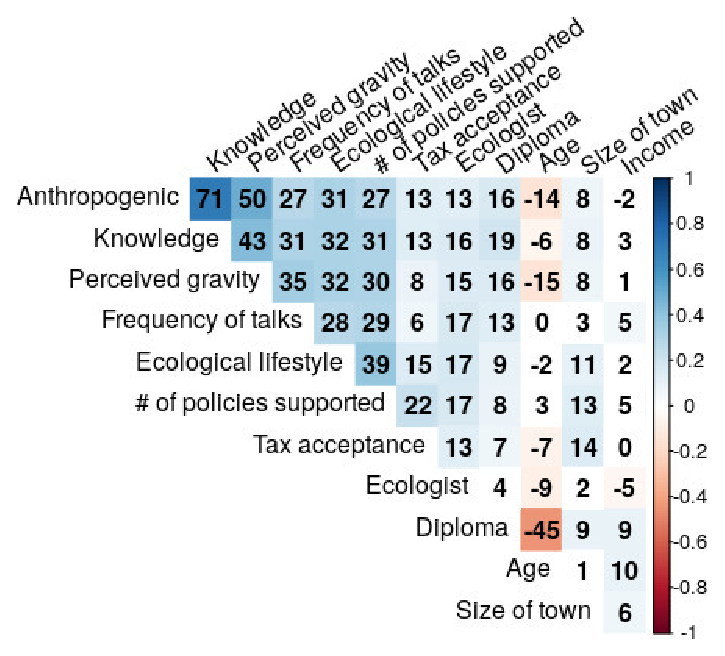
\includegraphics[width=0.95\columnwidth]{Images_EPS/correlation_matrix2.eps}
\caption{Correlations between attitudes over climate change, climate policies and socio-demographics (in \%).}
\label{fig:correlations}
\end{figure}

    \subsection{Attitudes over policies}\label{sec:determinants_attitudes_policies}

%
To better understand the heterogeneity in people's support, we regress several indicators of attitudes towards climate policies on respondents' characteristics. Table \ref{tab:politiques_env} reports the results for the acceptance of our Tax \& Dividend (columns 1-2) and the readiness to adopt an ecological lifestyle (6) in the case that the richest were contributing, efforts were shared globally, and alternatives were developed. We also use the eight policies proposed in Figure \ref{fig:policies} in our dependent variables: column 3 studies the share of policies approved while column 4 features the preference for norms vs. taxes within the policies. Similarly, column 5 uses six measures of Figure \ref{fig:recycling} to define an index of preference for earmarking vs. transfers. Indexes for these preferences are constructed as follows:

\begin{align}
\textnormal{Norms vs. taxes} = \sum_{p \in \textnormal{norms}} \textnormal{score}_{p} - \sum_{p \in \textnormal{taxes}}  \textnormal{score}_{p}
\label{eq:norms_vs_taxes}
\end{align}

\noindent
where the score of each measure corresponds to a grade between $-$2 (for a ``Not at all'' answer) and 2 (for ``Yes, completely''). We proceed similarly for earmarking vs. transfers, and describe the categorization of measures in Appendix \ref{app:measures}. Again, we normalize these two indexes by subtracting the mean (2.8 for norms vs. taxes, 1.4 for earmarking vs. transfers) and dividing by the standard deviation (3.3 and 3.1 respectively). Tables 3.2 and 3.3 in online Appendix provide the analysis of the determinants of acceptance for each of the eight policies and nine revenue recycling. The results are overall very similar to those provided by the more synthetic indicators presented here.

%


\begin{table*}[!htbp] \centering 
  \caption{Determinants of attitudes towards climate policies} 
  \label{tab:politiques_env} 
\makebox[\textwidth][c]{ \begin{tabular}{@{\extracolsep{5pt}}lcccccc} 
\\[-1.8ex]\hline 
\hline \\[-1.8ex] 
\\[-1.8ex] & \multicolumn{2}{c}{Acceptance of} & Share of policies & Norms & Earmarking & Ecological \\ \\[-1.8ex] & \multicolumn{2}{c}{Tax \& dividend} & approved & vs. taxes & vs. transfers & lifestyle \\ 
\\[-1.8ex] & (1) & (2) & (3) & (4) & (5) & (6)\\ 
\hline \\[-1.8ex] 
 Knowledge about CC & 0.029$^{***}$ & 0.048$^{***}$ & 0.044$^{***}$ & 0.024 & 0.131$^{***}$ & 0.103$^{***}$ \\ 
  & (0.009) & (0.009) & (0.005) & (0.020) & (0.020) & (0.009) \\ 
  CC is disastrous & 0.022 & 0.037$^{**}$ & 0.081$^{***}$ & 0.125$^{***}$ & 0.156$^{***}$ & 0.142$^{***}$ \\ 
  & (0.018) & (0.018) & (0.010) & (0.040) & (0.039) & (0.018) \\ 
  Interest in politics (0 to 2) & $-$0.019 &  & 0.034$^{***}$ & $-$0.010 & 0.053$^{*}$ & 0.026$^{**}$ \\ 
  & (0.013) &  & (0.007) & (0.029) & (0.028) & (0.013) \\ 
  Ecologist & 0.126$^{***}$ &  & 0.082$^{***}$ & $-$0.134$^{**}$ & 0.249$^{***}$ & 0.149$^{***}$ \\ 
  & (0.024) &  & (0.013) & (0.056) & (0.054) & (0.025) \\ 
  Yellow Vests: PNR & $-$0.021 &  & $-$0.052$^{***}$ & 0.007 & $-$0.110 & $-$0.079$^{**}$ \\ 
  & (0.032) &  & (0.018) & (0.073) & (0.071) & (0.033) \\ 
  Yellow Vests: understands & $-$0.144$^{***}$ &  & $-$0.029$^{**}$ & $-$0.056 & $-$0.091$^{*}$ & $-$0.013 \\ 
  & (0.022) &  & (0.012) & (0.050) & (0.049) & (0.022) \\ 
  Yellow Vests: supports & $-$0.222$^{***}$ &  & $-$0.048$^{***}$ & $-$0.131$^{**}$ & $-$0.142$^{***}$ & $-$0.023 \\ 
  & (0.023) &  & (0.013) & (0.053) & (0.052) & (0.024) \\ 
  Yellow Vests: is part & $-$0.214$^{***}$ &  & $-$0.084$^{***}$ & $-$0.252$^{***}$ & $-$0.175$^{*}$ & $-$0.037 \\ 
  & (0.043) &  & (0.023) & (0.097) & (0.095) & (0.043) \\ 
  Left-right: Extreme-left & $-$0.040 &  & 0.025 & $-$0.285$^{**}$ & 0.167 & 0.047 \\ 
  & (0.056) &  & (0.031) & (0.127) & (0.124) & (0.056) \\ 
  Left-right: Left & 0.072$^{***}$ &  & $-$0.005 & $-$0.137$^{**}$ & 0.002 & 0.028 \\ 
  & (0.027) &  & (0.015) & (0.061) & (0.060) & (0.027) \\ 
  Left-right: Center & 0.051$^{*}$ &  & 0.011 & $-$0.051 & 0.051 & 0.095$^{***}$ \\ 
  & (0.030) &  & (0.016) & (0.068) & (0.066) & (0.030) \\ 
  Left-right: Right & $-$0.022 &  & 0.008 & 0.030 & 0.064 & 0.005 \\ 
  & (0.028) &  & (0.016) & (0.065) & (0.063) & (0.029) \\ 
  Left-right: Extreme-right & $-$0.041 &  & $-$0.028 & 0.055 & 0.009 & 0.014 \\ 
  & (0.034) &  & (0.018) & (0.077) & (0.075) & (0.034) \\ 
  Diploma (1 to 4) & $-$0.006 & $-$0.001 & 0.005 & 0.006 & 0.017 & $-$0.008 \\ 
  & (0.009) & (0.008) & (0.005) & (0.020) & (0.020) & (0.009) \\ 
  Age: 25 -- 34 & $-$0.047 & $-$0.099$^{***}$ & $-$0.023 & 0.038 & $-$0.159$^{*}$ & 0.032 \\ 
  & (0.041) & (0.032) & (0.022) & (0.093) & (0.090) & (0.041) \\ 
  Age: 35 -- 49 & $-$0.047 & $-$0.089$^{***}$ & $-$0.017 & 0.189$^{**}$ & $-$0.002 & 0.039 \\ 
  & (0.040) & (0.030) & (0.022) & (0.092) & (0.089) & (0.041) \\ 
  Age: 50 -- 64 & $-$0.054 & $-$0.114$^{***}$ & $-$0.010 & 0.322$^{***}$ & $-$0.058 & 0.049 \\ 
  & (0.044) & (0.031) & (0.024) & (0.100) & (0.097) & (0.044) \\ 
  Age: $\geq$ 65 & $-$0.066 & $-$0.100$^{***}$ & $-$0.009 & 0.370$^{***}$ & $-$0.056 & 0.008 \\ 
  & (0.052) & (0.032) & (0.028) & (0.118) & (0.115) & (0.052) \\ 
  Income (k\euro{}/month) & 0.006 & 0.001 & 0.009$^{**}$ & 0.014 & 0.031$^{*}$ & $-$0.004 \\ 
  & (0.008) & (0.005) & (0.004) & (0.018) & (0.017) & (0.008) \\ 
  Sex: Male & $-$0.053$^{***}$ & $-$0.074$^{***}$ & $-$0.017$^{*}$ & $-$0.028 & $-$0.004 & $-$0.063$^{***}$ \\ 
  & (0.018) & (0.017) & (0.010) & (0.040) & (0.039) & (0.018) \\ 
  Size of town (1 to 5) & 0.019$^{**}$ & 0.033$^{***}$ & 0.0002 & 0.009 & $-$0.003 & $-$0.003 \\ 
  & (0.008) & (0.007) & (0.004) & (0.018) & (0.017) & (0.008) \\ 
  Frequency of public transit & $-$0.003 & 0.014$^{**}$ & $-$0.003 & 0.046$^{***}$ & 0.021 & 0.024$^{***}$ \\ 
  & (0.007) & (0.006) & (0.004) & (0.017) & (0.016) & (0.007) \\ 
 \hline \\[-1.8ex] 
Additional covariates & \checkmark & & \checkmark  & \checkmark & \checkmark & \checkmark  \\  &  &  &  &  &  &  \\ 
Observations & 3,002 & 3,002 & 3,002 & 3,002 & 3,002 & 3,002 \\ 
R$^{2}$ & 0.150 & 0.051 & 0.226 & 0.081 & 0.121 & 0.202 \\ 
\hline 
\hline \\[-1.8ex] 
\uline{Note:}  & \multicolumn{6}{r}{$^{*}$p$<$0.1; $^{**}$p$<$0.05; $^{***}$p$<$0.01} \\ 
\end{tabular} 
} \\ \quad \\ {\footnotesize \textsc{Note:} Standard errors are reported in parentheses. Omitted variables are \uline{Yellow Vests: opposes}, \uline{Age : 18 -- 24} and \uline{Left-right: Indeterminate}. Additional covariates are defined in \ref{app:covariates}.} \end{table*} 

As suggested by the correlation matrix of section \ref{sec:determinants_attitudes_CC}, knowledge about CC and the conviction that it would be disastrous positively affect the approval of climate policies, \uline{ceteris paribus}. Excluding the (endogenous) variables describing political orientation, an increase in knowledge by 1 s.d. would induce a lower likelihood to reject Tax \& Dividend by 5 p.p. (column 2). The effect of these variables is even stronger when considering the share of policies approved: controlling for socio-demographics, an increase in knowledge by 1 s.d. is associated with an additional approval of 6 p.p. while the conviction that CC is disastrous increases it by 9 p.p. (see online Appendix 3.4). Beyond the strong correlation we previously found, these results confirm that increasing climate awareness could significantly increase the support for climate policies. %

%
%
%
%
Besides attitudes over CC, the two most critical determinants appear to be one's affiliation as an ecologist and one's position towards the Yellow Vests. All else equal, ecologists are more likely to accept Tax \& Dividend by 13 p.p., and more willing to approve other environmental policies by about 8 p.p. Conversely, holding other variables constant, people supporting the Yellow Vests are 22 p.p. more likely to reject Tax \& Dividend relative to those opposed to the movement. As shown in column 3, higher affinity with the Yellow Vests is also associated with less support for other climate policies. Ecologists (resp. the Yellow Vests supporters) being more (resp. less) favorable to environmental policies and spending, their relative preference for earmarking vs. transfers is higher (resp. lower) than average, while for both groups the relative preference for norms vs. taxes is lower than average. Also, ecologists' attitudes towards environmental policies translate into a higher willingness to adopt an ecological lifestyle (by 15 p.p.), but the opposite does not hold true for the Yellow Vests. Although this could signal some warm glow,\footnote{Here, ``warm glow'' refers to one's unintentional strategy to overestimate their virtue in order to derive satisfaction.} it also suggests that their strong rejection of environmental policies does not simply reflect lower concerns about the environment. Rather, the conditions of fairness embedded in our question could be critical for Yellow Vests to accept sacrifices. Their rejection could also reflect a deeper rejection of policies in general, due to a high distrust in the government --- documented in \citet{algan_et_al_19}. This interpretation echoes the recent findings of \citet{rafaty_perceptions_2018}, who shows that perceptions of corruption and political distrust negatively affect the stringency of climate policies. Finally, although the heterogeneity in responses is significant between these two groups, the ranking of the preferred option remains consistent: on average, both ecologists and supporters of the Yellow Vests favor norms over taxes and earmarking over transfers. 
%

%
%

%

%

%
%
A parallel message from Table \ref{tab:politiques_env} is that the standard left-right spectrum is not the most relevant to understand attitudes towards environmental policies. None of our five left-right dummy variables are significantly correlated with the share of policies approved, and overall, attitudes vary much less along the left-right spectrum than along the Yellow Vests cleavage. That being said, Tax \& Dividend is still significantly more supported by people from the left (+7 p.p.) and the center (+5 p.p.) than by those indeterminate. This is in line with the literature (see e.g. \citealt{bornstein_lanz_2008,mccright_increasing_2013} or \citealt{drews_van_der_bergh_2016} for a review). Without controlling for other variables, we find that people that are most likely to accept the Tax \& Dividend in France are the ones affiliated with the center (+9 p.p. relative to ``Indeterminate''), and the least likely are those on the extreme-right (-15 p.p., see online Appendix 3.4), which may be driven by their respective support or rejection of the current government who tried to increase the carbon tax. Our results also show that people from the extreme-left and the center are the most likely to approve other environmental policies (+7 p.p.), while the least likely are those on the extreme-right ($-$6 p.p.). Still, these differences become small and not statistically significant when covariates are included. %
%

%
%

Besides political attitudes, we also observe heterogeneity in people's responses along socio-demographic lines. As in attitudes over CC, age plays a role, as 18-24 are about 10 p.p. more likely to accept the Tax \& Dividend (column 2). Still, controlling for knowledge, political attitudes and other variables, this effect is reduced by half. Similarly, more educated people tend to be more open to environmental policies \citep[as previously found by][]{thalmann_public_2004}, but this effect becomes insignificant once age dummies are included as covariates. Furthermore, we find little effect of income on attitudes towards climate policies, a result that confirms that of \citet{thalmann_public_2004} in Switzerland. Using our full set of controls, the most significant variables differ from the main factors of attitudes over CC: these significant variables are size of town \citep[city dwellers being more favorable to environmental policies, as in][]{thalmann_public_2004}, and sex (males being less favorable). Although men have a higher knowledge about CC than women on average, this does not translate into higher pessimism (see section \ref{sec:determinants_attitudes_CC}), and it even coincides with lower support for climate policies. This phenomenon is consistent with the findings of \citet{stern_value_1993} and \citet{hampel_gender_1996} that women are more attentive to links between the environment and things they value, even if they share the same values and beliefs as men. Difference in perception of CC's impact on oneself could explain women's higher support for climate policies, even given a lower factual knowledge. %

%

%

%

%

%

%

%

\section{Conclusion}\label{sec:conclusion}

%

%
%
Despite a social movement against the carbon tax, French people appear mostly aware and concerned about climate change. Their rejection should therefore not be taken as a low willingness to act for the environment, but rather as a perceived inadequacy between current carbon taxation and the fight for the climate. Our results identify several barriers --- distributive concerns, inefficacy and lack of alternatives --- that could be partly alleviated with specific complementary policies. In particular, French people favor investments in green infrastructures that provide them with alternatives and foster the energy transition. They also appear willing to accept certain norms as well as Pigouvian taxes if these target specific behaviors (or populations) such as air travel. The heterogeneity in people's attitudes is significant, but the relative ranking of the different policy options are in general consistent across groups of population, suggesting the following paths towards a successful ecological transition.
%
%


%
First and foremost, a massive and long-lasting information campaign could be launched to improve knowledge about climate change and climate policies. Indeed, higher knowledge is clearly associated with higher concern for CC and higher support for climate policies. Second, as people mostly favor policies that provide alternatives to fossil fuels, the government could develop such policies as a substitute to a carbon tax: investments, subsidies, and regulations in favor of public transport, cleaner vehicles and thermal insulation, etc. Third, a tax and dividend restricted to kerosene could serve as a learning example as kerosene taxation is popular.\footnote{\citet{murray_british_2015} document an increase in the support of the carbon tax following its implementation in British Columbia.} Last but not least, a more cost-effective carbon tax should later complement these policies, as people get convinced by the objective of carbon neutrality and by the government's commitment towards this goal. 

But to successfully introduce a carbon tax, it is important to build public trust in politicians \citep{harring_jagers_2013,rafaty_perceptions_2018} and to correct the inequities of the tax. As such, it is no surprise if political trust is among the highest in the country that first introduced a carbon tax, Sweden \citep{klenert_making_2018}. It is no coincidence either if the 1991 Swedish tax was part of a comprehensive restructuring of the tax system, the popular ``reform of the century'', resulting from a dialogue with all stakeholders \citep{sterner_environmental_2014}. 

The French government is willing to build such a democratic consensus, as it has just launched an assembly to tackle climate change composed of 150 citizens randomly drawn. Nevertheless, it will remain challenging to reintroduce a carbon-tax in the short-run, since French people's beliefs about carbon taxation are largely biased, and these biases are well anchored (as shown in our companion paper, \citealt{douenne_can_2019}). In a nutshell, market imperfections, distributive effects and political acceptability concerns all call for a combination of different types of climate policies rather than a single price signal \citep{stern_report_2017,stiglitz_addressing_2019}. The French context seems to call for a focus on the former to make the latter politically acceptable. 

%

%

%

%

%

%

%
%

%

%


\paragraph*{Acknowledgments} We are grateful to Mouez Fodha, Fanny Henriet and Katheline Schubert for their comments and their help to get funding. We also thank Stefano Carattini, Mathias Lé, seminar participants at the Paris School of Economics, an anonymous referee of the FAERE Working Paper series and two anonymous referees of this journal. We are thankful to Christina Hobbs for the proof-reading. We would also like to show our gratitude to Stefanie Stantcheva, Michael I. Norton and the Harvard Business School for allowing us to use their Qualtrics account. We are grateful to Christina Hobbs for the proof-reading. We acknowledge financial support from the Cepremap, EUR PGSE (ANR-17-EURE-0001), ANR (ANR16-CE03-0011), and Université Paris 1 Panthéon-Sorbonne economics doctoral school (ED 465).

%

\newpage
%
\bibliographystyle{plainnat_no_url_no_note}%
\bibliography{CO2_tax_acceptability}

%

%
%
%
%
%
%
%
%
%
%

%

%
%
\begin{appendices}
\addtocontents{toc}{\setcounter{tocdepth}{1}}
\renewcommand{\thetable}{\Alph{section}.\arabic{table}}

\section{Raw data\label{app:Raw-Data}}

\begin{table}[!htbp]
\label{table:sample_characteristics}
\caption{\label{tab:Sample-Characteristics}Sample characteristics: quotas stratas.}
\centering
\begin{tabular}{lcc}
\hline \hline  \\[-1.8ex]
 & \uline{Population} & Sample  \tabularnewline \\[-1.8ex]
\hline  \\[-1.8ex]
\textbf{gender} & & \tabularnewline  \\[-1.8ex]
woman & \uline{0.52} & 0.53\tabularnewline
man & \uline{0.48} & 0.47\tabularnewline
\hline \\[-1.8ex]
\textbf{age} &  & \tabularnewline  \\[-1.8ex]
18-24 & \uline{0.12} & 0.11\tabularnewline
25-34 & \uline{0.15} & 0.11\tabularnewline
35-49 & \uline{0.24} & 0.24\tabularnewline
50-64 & \uline{0.24} & 0.26\tabularnewline
>65 & \uline{0.25} & 0.27\tabularnewline
\hline \\[-1.8ex]
\textbf{profession} &  & \tabularnewline  \\[-1.8ex]
farmer & \uline{0.01} & 0.01\tabularnewline
independent & \uline{0.03} & 0.04\tabularnewline
executive & \uline{0.09} & 0.09\tabularnewline
intermediate & \uline{0.14} & 0.14\tabularnewline
employee & \uline{0.15} & 0.16\tabularnewline
worker & \uline{0.12} & 0.13\tabularnewline
retired & \uline{0.33} & 0.33\tabularnewline
inactive & \uline{0.12} & 0.11\tabularnewline
\hline  \\[-1.8ex]
\textbf{education} &  & \tabularnewline  \\[-1.8ex]
No diploma or \uline{Brevet} & \uline{0.30} & 0.24\tabularnewline
\uline{CAP} or \uline{BEP} & \uline{0.25} & 0.26\tabularnewline
\uline{Baccalauréat} & \uline{0.17} & 0.18\tabularnewline
Higher & \uline{0.29} & 0.31\tabularnewline
\hline  \\[-1.8ex]
\textbf{size of town} &  & \tabularnewline  \\[-1.8ex]
rural & \uline{0.22} & 0.24\tabularnewline
<20k & \uline{0.17} & 0.18\tabularnewline
20-99k & \uline{0.14} & 0.13\tabularnewline
>100k & \uline{0.31} & 0.29\tabularnewline
Paris area & \uline{0.16} & 0.15\tabularnewline
\hline  \\[-1.8ex]
\textbf{region} &  & \tabularnewline  \\[-1.8ex]
\uline{IDF} & \uline{0.19} & 0.17\tabularnewline
 \uline{Nord} & \uline{0.09} & 0.10\tabularnewline
 \uline{Est} & \uline{0.13} & 0.12\tabularnewline
\uline{SO} & \uline{0.09} & 0.09\tabularnewline
\uline{Centre} & \uline{0.10} & 0.12\tabularnewline
 \uline{Ouest} & \uline{0.10} & 0.10\tabularnewline
 \uline{Occ} & \uline{0.09} & 0.09\tabularnewline
\uline{ARA} & \uline{0.12} & 0.13\tabularnewline
\uline{PACA} & \uline{0.09} & 0.09\tabularnewline  \\[-1.8ex]
\hline \hline 
\end{tabular}\bigskip{}
\end{table}


\begin{table}[!htbp]
    \caption{Households' characteristics.\label{tab:app-energetic-characs}}
\centering
\begin{tabular}{lcc}
\hline \hline  \\[-1.8ex]
 & \uline{Population} & Sample  \tabularnewline \\[-1.8ex]
\hline  \\[-1.8ex]
\multicolumn{3}{l}{\textbf{Household composition (mean)}} \tabularnewline  \\[-1.8ex]
Household size & \uline{2.36} & 2.38\tabularnewline
Number of adults & \uline{2.03} & 1.93\tabularnewline
c.u. & \uline{1.60} & 1.61\tabularnewline
\hline   \\[-1.8ex]
\multicolumn{3}{l}{\textbf{Energy source (share)}} \tabularnewline  \\[-1.8ex]
Gas & \uline{0.42} & 0.36\tabularnewline
Fuel & \uline{0.12} & 0.09\tabularnewline
\hline   \\[-1.8ex]
\multicolumn{3}{l}{\textbf{Accomodation size (m$^\textnormal{2}$)}} \tabularnewline  \\[-1.8ex]
mean & \uline{97} & 96\tabularnewline
p25 & \uline{69} & 66\tabularnewline
p50 & \uline{90} & 90\tabularnewline
p75 & \uline{120} & 115\tabularnewline
\hline   \\[-1.8ex]
\multicolumn{3}{l}{\textbf{Distance traveled by car (km/year)}} \tabularnewline  \\[-1.8ex]
mean & \uline{13,735} & 15,328\tabularnewline
p25 & \uline{4,000} & 4,000\tabularnewline
p50 & \uline{10,899} & 10,000 \tabularnewline
p75 & \uline{20,000 } & 20,000 \tabularnewline
\hline   \\[-1.8ex]
\multicolumn{3}{l}{\textbf{Fuel economy (L/100 km)}} \tabularnewline  \\[-1.8ex]
mean & \uline{6.39} & 7.25\tabularnewline
p25 & \uline{6} & 5\tabularnewline
p50 & \uline{6.5} & 6\tabularnewline
p75 & \uline{7.5} & 7\tabularnewline  \\[-1.8ex]
\hline \hline 
\end{tabular}\bigskip{}

%
     \footnotesize{\textsc{Sources:} Matched BdF; except for number of adults (ERFS) and domestic fuel (\href{https://www.lesechos.fr/industrie-services/energie-environnement/le-chauffage-au-fioul-devient-de-plus-en-plus-cher-147372}{CEREN}).}
\end{table}

\section{Sources on GhG emissions\label{app:sources}}

\subsection{Carbon footprints\label{app:footprint}}

\paragraph{Plane vs. train}

Given that French electricity mix is decarbonized at 93\%\footnote{Cf. \href{https://www.rte-france.com/sites/default/files/be_pdf_2018v3.pdf}{RTE - Bilan électrique 2018} (p. 32).}, the carbon footprint of highspeed train is actually more than 20 times lower than that of an interior flight of the same distance. Hence, we chose Bordeaux - Nice as our case study as the train connection makes a big detour by Paris. Thus, we obtain an emission of 10 kg of CO$_\textnormal{2}$ by train as compared to 180 kg by plane. Our source for train is the French railroad company, \href{https://www.oui.sncf/aide/calcul-des-emissions-de-co2-sur-votre-trajet-en-train}{SNCF}, and is consistent with data aggregated by the official agency \href{basecarbone.fr}{ADEME}. For the flight, our source is a  \href{https://calculator.carbonfootprint.com/calculator.aspx?tab=3}{carbon footprint calculator}. \href{http://www.climatecare.org/home.aspx}{Another calculator} provides almost the same result, so we preferred this figure rather than a higher figure from a \href{https://co2.myclimate.org/fr/flight_calculators}{third calculator}.

\paragraph{Nuclear vs. wind}

AR5 from \citet{ar5_ar5_nodate} and \citet{pehl_understanding_2017} show that nuclear power plants and wind turbines have similar carbon footprint, at 10 gCO$_\textnormal{2}$eq$/$kWh (for comparison, it is 500 for gas combined cycle).

\paragraph{Beef vs. pasta}

\citet{poore_reducing_2018} show that median beef carbon footprint is 60 kgCO$_\textnormal{2}$eq$/$kg (more precisely, 30 kgCO$_\textnormal{2}$eq per 100g of protein and 200g of protein per kg); while the carbon footprint of wheat pasta is 1.3 kgCO$_\textnormal{2}$eq$/$kg (0.5 kgCO$_\textnormal{2}$eq per 1000 kcal of protein and 2695 kcal per kg). Given that a beef steak \href{http://www.lessentieldesviandes-pro.org/introduction.php}{weighs 100-125g}, its carbon footprint is twenty times that of two servings of pasta of 125g each. 

\subsection{Current and target emissions\label{app:emission}}

French consumption-based yearly GhG emissions amounted in 2014 to 712 MtCO$_\textnormal{2}$eq, i.e. 10.8 tCO$_\textnormal{2}$eq p.c., and are roughly stable in recent years \citep{cgdd_chiffres_2019}. To stop climate change and stabilize the GhG concentration in the atmosphere, it is required to meet zero net emissions. To meet the Paris agreement,  \href{https://www.ecologique-solidaire.gouv.fr/strategie-nationale-bas-carbone-snbc}{France National Low-Carbon Strategy} aims to achieve carbon (i.e. GhG) neutrality by 2050 \citep{ministry_of_ecology_france_2015}. Given carbon sinks estimated at 85 Mt$_\textnormal{2}$eq for 2050 (mainly forest and soil), this strategy requires to reach gross emissions of about 1 tCO$_\textnormal{2}$eq p.c. at this date. Admittedly, less stringent scenarios may still allow to keep global warming below +2\textdegree{}C in 2100 with good probability --- even considering the same burden share for France --- by relying more heavily on net negative emissions after 2070 through carbon capture and storage. For this reason, we consider a range of answers as correct for the French target emission in 2050: from 0 to 2 tCO$_\textnormal{2}$eq p.c.

%

%
%
%
%
%
%
%
%
%
%
%
%
%
%
%
%
%
%
%
%
%
%



%
%
%
%
%
%
%
%
%
%
%
%
%
%
%
%
%
%
%
%
%
%
%
%
%
%
%
%
%
%
%
%
%
%
%
%
%
%
%
%
%
%
%
%
%
%
%
%
%
%
%
%
%
%
%
%
%

\section{Details on main regressions}
\subsection{Control variables\label{app:covariates}}

Our regression Tables \ref{tab:determinants_attitudes_CC} and \ref{tab:politiques_env} display only the most relevant variables, but --- when specified --- the following additional covariates are included as controls:

\subparagraph{Socio-demographics:} \uline{respondent's income; household's income; employment status \textnormal{(9 categories)}; socio-professional category \textnormal{(8 categories)}; region of France \textnormal{(10 categories)}; household size; number of people above 14; number of adults; single; number of c.u.; smokes; favored medium for news \textnormal{(5 categories)}.}

\subparagraph{Political orientation:} \uline{conservative; liberal; humanist; patriot; apolitical.}

\subparagraph{Energy and exposure to policies:} \uline{heating energy: gaz; heating energy: domestic fuel; accomodation size; annual distance travelled by car; fuel economy; type of fuel: diesel; type of fuel: gasoline; number of vehicles; simulated net gain from Tax \& Dividend; opinion on public transports; mode of commuting transport.}

\subsection{Measures for relative preferences\label{app:measures}}

We constructed the two indexes of section \ref{sec:determinants_attitudes_policies} using the following measures:

\subparagraph{Norms:} \uline{insulation standards;  pollution standards; roadworthiness standards; prohibition of polluting vehicles.}

\subparagraph{Taxes:} \uline{kerosene; red meat; urban tolls; climate fund.}

\subparagraph{Earmarking:} \uline{renovation; renewables; non polluting transport.}

\subparagraph{Transfers:} \uline{to bottom half; to all; to constrained households.}

%
\section{Questionnaire\label{app:questionnaire}}

Hereafter, we only describe questions of the survey that are used
in the present paper. The other questions are described and analyzed
in our companion paper \citep{douenne_can_2019}. Words that appear in bold were actually in both bold and underlined in the respondents' questionnaire.

\paragraph{Socio-demographics}
\begin{enumerate}[resume,leftmargin=*]
\item What is your postal code? 
\item What is your gender (in the sense of civil status)? \uline{}\\
\uline{Female; Male }
\item What is your age group? \uline{}\\
\uline{18 to 24 years old; 25 to 34 years old; 35 to 49 years old;
50 to 64 years old; 65 years old or more} 
\item What is your employment status? \uline{}\\
\uline{Permanent; Temporary contract; Unemployed; Student; Retired;
Other active; Inactive}
\item What is your socio-professional category? (Remember that the unemployed
are active workers). \uline{}\\
\uline{Farmer; Craftsperson, merchant; Independent; Executive; Intermediate
occupation; Employee; Worker; Retired; Other Inactive} 
\item What is your highest degree? \uline{}\\
\uline{No diploma; Brevet des collèges; CAP or BEP {[}secondary{]};
Baccalaureate; Bac +2 (BTS, DUT, DEUG, schools of health and social
training...); Bac +3 (licence...) {[}bachelor{]}; Bac +5 or more (master,
engineering or business school, doctorate, medicine, master, DEA,
DESS...)}
\item How many people live in your household? Household includes: you, your
family members who live with you, and your dependents. 
\item What is your net \textbf{\textbf{monthly}} income (in euros)? \textbf{\textbf{All
income}} (before withholding tax) is included here: salaries, pensions,
allowances, APL {[}housing allowance{]}, land income, etc. 
\item What is the net \textbf{\textbf{monthly}} income (in euros) \textbf{\textbf{of
your household}}? \textbf{\textbf{All income}} (before withholding
tax) is included here: salaries, pensions, allowances, APL {[}housing
allowance{]}, land income, etc. 
\item In your household how many people are 14 years old or older (\textbf{\textbf{including
yourself}})? 
\item In your household, how many people are over the age of majority (\textbf{\textbf{including
yourself}})? 
\end{enumerate}

\paragraph{Energy characteristics}
\begin{enumerate}[resume,leftmargin=*]
\item What is the surface area of your home? (in m\texttwosuperior )
\item What is the heating system in your home? \uline{}\\
\uline{Individual heating; Collective heating; PNR (Don't know, don't
say)}
\item What is the main heating energy source in your home? \uline{}\\
\uline{Electricity Town gas; Butane, propane, tank gas; Heating oil;
Wood, solar, geothermal, aerothermal (heat pump); Other; PNR (Don't
know, don't say)}
\item How many motor vehicles does your household have? \uline{}\\
\uline{None; One; Two or more} 
\item {[}Without a vehicle{]} How many kilometers have you driven in the
last 12 months? 
\item {[}One vehicle{]} What type of fuel do you use for this vehicle? \uline{}\\
\uline{Electric or hybrid; Diesel; Gasoline; Other} 
\item {[}One vehicle{]} What is the average fuel economy of your vehicle?
(in Liters per 100 km)
\item {[}One vehicle{]} How many kilometers have you driven with your vehicle
in the last 12 months?
\item {[}At least two vehicles{]} What type of fuel do you use for your
main vehicle?\\
 \uline{Electric or hybrid; Diesel; Gasoline; Other} 
\item {[}At least two vehicles{]} What type of fuel do you use for your
second vehicle?\\
 \uline{Electric or hybrid; Diesel; Gasoline; Other} 
\item {[}At least two vehicles{]} What is the average fuel economy of all
your vehicles? (in Liters per 100 km) 
\item {[}At least two vehicles{]} How many kilometers have you driven with
all your vehicles in the last 12 months? 
\end{enumerate}

\paragraph{Partial reforms {[}transport / housing{]}}

(...)\uline{}
\begin{enumerate}[resume,leftmargin=*]
\item If fuel prices increased by 50 cents per liter, by how much would
\textbf{\textbf{your household}} reduce its fuel consumption? \uline{}\\
\uline{0\% -} {[}\uline{I already consume almost none }/\uline{ I am
already not consuming}{]}\uline{; 0\% - }{[}\uline{I am constrained
on all my trips} / \uline{I will not reduce it}{]}\uline{; From 0\%
to 10\%; From 10\% to 20\%; From 20\% to 30\%; More than 30\% - }{[}\uline{I
would change my travel habits significantly }/ \uline{I would change
my consumption significantly}{]}
\item In your opinion, if {[}fuel prices increased by 50 cents per liter
/ gas and heating oil prices increased by 30\%{]}, by how much would
\textbf{\textbf{French people}} reduce their consumption on average?
\uline{}\\
\uline{From 0\% to 3\%; From 3\% to 10\%; From 3\% to 10\%; From 10\%
to 20\%; From 20\% to 30\%; More than 30\%} 
\end{enumerate}

\paragraph{Tax \& Dividend: initial}
\begin{enumerate}[resume,leftmargin=*]
\item The government is studying an increase in the carbon tax, whose revenues
would be redistributed to all households, regardless of their income.
This would imply: 
\end{enumerate}
\begin{itemize}
\item an increase in the price of gasoline by 11 cents per liter and diesel
by 13 cents per liter; 
\item an increase of 13\% in the price of gas, and 15\% in the price of
heating oil;
\item an annual payment of 110\euro{} to each adult, or 220\euro{} per year for a couple.
\\
\\
(...)
\end{itemize}
\begin{enumerate}[resume,leftmargin=*]
\item {[} {[}empty{]} / Scientists agree that a carbon tax would be effective
in reducing pollution.{]} Do you think that such a measure would reduce
pollution and fight climate change? \uline{}\\
\uline{Yes; No; PNR (Don't know, don't say)}
\item In your opinion, which categories would lose {[} {[}blank{]} / purchasing
power{]} with such a measure? (Several answers possible) \uline{}\\
\uline{No one; The poorest; The middle classes; The richest; All French
people; Rural or peri-urban people; Some French people, but not a
particular income category; PNR (Don't know, don't say)} 
\item In your opinion, what categories would gain purchasing power with
such a measure? (Several answers possible) \uline{}\\
\uline{No one; The poorest; The middle classes; The richest; All French
people; Urban dwellers; Some French people, but not a particular income
category; PNR (Don't know, don't say)} 
\end{enumerate}

\paragraph{Tax \& Dividend: after knowledge}

We always consider the same measure. (...)
\begin{enumerate}[resume,leftmargin=*]
\item Why do you think this measure is beneficial? (Maximum three responses)
\uline{}\\
\uline{Contributes to the fight climate change; Reduces the harmful
effects of pollution on health; Reduces traffic congestion; Increases
my purchasing power; Increases the purchasing power of the poorest;
Fosters France's independence from fossil energy imports; Prepares
the economy for tomorrow's challenges; For none of these reasons;
Other (specify): }
\item Why do you think this measure is unwanted? (Maximum three answers)
\uline{}\\
\uline{Is ineffective in reducing pollution; Alternatives are insufficient
or too expensive; Penalizes rural areas; Decreases my purchasing power;
Decreases the purchasing power of some modest households; Harms the
economy and employment; Is a pretext for raising taxes; For none of
these reasons; Other (specify):} 
\end{enumerate}
(...)

\paragraph{Attitudes over other policies}
\begin{enumerate}[resume,leftmargin=*]
\item In which cases would you be in favor of increasing the carbon tax?
I would be in favor if the tax revenues were used to finance...\uline{ }
\begin{enumerate}[resume,leftmargin=*]
\item a payment to the 50\% poorest French people (those earning less than
1670\euro{} per month) 
\item a payment to all French people 
\item a compensation for households forced to consume petroleum products
\item a decrease in social contributions
\item a decrease in VAT 
\item a decrease in the public deficit 
\item the thermal renovation of buildings 
\item renewable energy (wind, solar, etc.) 
\item clean transport
\end{enumerate}
\end{enumerate}
\uline{Yes, absolutely; Yes, rather; Indifferent or Don't know; No,
not really; No, not at all}
\begin{enumerate}[resume,leftmargin=*]
\item Please select ``A little'' (test to check that you are attentive).
\uline{}\\
\uline{Not at all; A little; A lot; Completely; PNR (Don't know, don't
say)} 
\item Would you support the following environmental policies? 
\begin{enumerate}[resume,leftmargin=*]
\item A tax on kerosene (aviation) 
\item A tax on red meat 
\item Stricter standards on the insulation of new buildings 
\item Stricter standards on the pollution of new vehicles
\item Stricter standards on pollution during roadworthiness tests 
\item The prohibition of polluting vehicles in city centers 
\item The introduction of urban tolls 
\item A contribution to a global climate fund 
\end{enumerate}
\end{enumerate}
\uline{Yes, absolutely; Yes, rather; Indifferent or Don't know; No,
not really; No, not at all}
\begin{enumerate}[resume,leftmargin=*]
\item For historical reasons, diesel is taxed less than gasoline. Would
you be in favor of raising taxes on diesel to catch up with the level
of taxation on gasoline? \uline{}\\
\uline{Yes; No; PNR (Don't know, don't say) }
\end{enumerate}

\paragraph{Attitudes over climate change}
\begin{enumerate}[resume,leftmargin=*]
\item How often do you talk about climate change? \uline{}\\
\uline{Several times a month; Several times a year; Almost never; PNR
(Don't know, don't say) }
\item In your opinion, climate change... \uline{}\\
\uline{is not a reality; is mainly due to natural climate variability;
is mainly due to human activity; PNR (Don't know, don't say). }
\item Which of the following elements contribute to global warming? (Several
answers possible) \uline{}\\
\uline{CO$_{2}$; Methane; Oxygen; Particulate matter}
\item In your opinion, which of the following statements are true? (Several
answers possible). \uline{}\\
\uline{Consuming one beef steak emits about 20 times more greenhouse
gases than eating two servings of pasta.; Electricity produced by
nuclear power emits about 20 times more greenhouse gases than electricity
produced by wind turbines.; A seat in a Bordeaux - Nice journey emits
about 20 times more greenhouse gases by plane than by high speed train. }
\item In your opinion, how would the effects of climate change be, if humanity
did nothing to limit it? \uline{}\\
\uline{Insignificant, or even beneficial; Small, because humans would
be able to live with it; Grave, because there would be more natural
disasters; Disastrous, lifestyles would be largely altered; Cataclysmic,
humankind would disappear; PNR(Don't know, don't say) }
\item In which of these two regions do you think will climate change have
the worst consequences? \uline{}\\
\uline{The European Union; India; As much in both }
\item In your opinion, in France, which generations will be seriously affected
by climate change? (Several answers possible) \uline{}\\
\uline{People born in the 1960s; People born in the 1990s; People born
in the 2020s; People born in the 2050s; None of the four }
\item In your opinion, who is responsible for climate change? (Several possible
choices) \uline{}\\
\uline{Each of us; The richest; Governments; Some foreign countries;
Past generations; Natural causes }
\item Currently, each French person emits on average the equivalent of 10
tons of CO$_{2}$ per year. \\
\\
In your opinion, how much must this figure be reduced to by 2050 in
order to hope to contain global warming to +2°C in 2100 (if all countries
did the same)? In 2050, we should emit at most... \uline{}\\
\uline{0; 1; 2; 3; 4; 5; 6; 7; 8; 9; 10} tons 
\item Has climate change had or will it have an influence on your decision
to make a child (or children)?\uline{ }\\
\uline{Yes; No; PNR (Don't know, don't say)}
\item {[}If \uline{Yes}{]} Why does climate change influence your decision
to have a child (or children)? (Several answers possible). \uline{}\\
\uline{Because I don't want my child to live in a devastated world.;
Because each additional human being aggravates climate change.}
\item Would you be willing to change your lifestyle to fight climate change?
(Several answers possible) \uline{}\\
\uline{Yes, if policies went in this direction; Yes, if I had the financial
means; Yes, if everyone did the same; No, only the richest people
have to change their way of life; No, it is against my personal interest;
No, I think climate change is not a real problem; I have already adopted
a sustainable way of life; I try, but I have trouble changing my habits} 
\item Assuming that all states in the world agree to firmly fight climate
change, notably through a transition to renewable energy, by making the richest contribute, and imagining that France would expand the
supply of non-polluting transport very widely; would you be willing
to adopt an ecological lifestyle (i.e. eat little red meat and ensure
to use almost no gasoline, diesel or kerosene)? \uline{}\\
\uline{Yes; No; PNR (Don't know, don't say) }
\end{enumerate}

%

%
%
%
%
%
%
%
%
%
%
%
%
%
%
%
%
%
%
%
%
%
%

\paragraph{Access to public transport and mobility habits}
\begin{enumerate}[resume,leftmargin=*]
\item How many minutes walk is it to the nearest public transit stop? (To
simplify, you can use the conversion 1 km = 10 min walk). \uline{}\\
\uline{in min:} ; \uline{PNR (Don't know, don't say) }
\item How often does the nearest public transport pass? (excluding school
buses) \uline{}\\
\uline{Less than three times a day; Between four times a day and once
an hour; Once or twice an hour; More than three times an hour; PNR
(Don't know, don't say) }
\item What do you think about the availability of public transport where
you live? It is... \uline{}\\
\uline{Satisfactory; Suitable, but should be increased; Limited, but
sufficient; Insufficient; PNR (Don't know, don't say) }
\item What mode of transportation do you mainly use for each of the following
trips?
\begin{enumerate}[resume,leftmargin=*]
\item Home - work (or studies) 
\item Grocery shopping 
\item Leisure (excluding holidays) 
\end{enumerate}
\end{enumerate}
\uline{Car; Public transport; Walking or cycling; Two-wheeled vehicle;
Carpooling;} \uline{Not concerned} 
\begin{enumerate}[resume,leftmargin=*]
\item {[}If \uline{Car }selected for Work{]} Would it be possible for you,
without changing your home or workplace, to travel from home to work
using public transport? \uline{}\\
\uline{Yes, it would not be very difficult for me; Yes, but it would
bother me; No; PNR (Don't know, don't say) }
\item {[}If \uline{Car }selected for Work{]} Would it be possible for you,
without changing your home or workplace, to travel from home to work
by walking or cycling? \uline{}\\
\uline{Yes, it would not be very difficult for me; Yes, but it would
bother me; No; PNR (Don't know, don't say) }
\end{enumerate}

\paragraph{Politics and media}
\begin{enumerate}[resume,leftmargin=*]
\item How much are you interested in politics? \uline{}\\
\uline{Almost not; A little; A lot }
\item How would you define yourself? (Several answers possible) \uline{}\\
\uline{Extreme left; Left; Center; Right; Extreme right; Liberal; Conservative;
Humanist; Patriot; Apolitical; Ecologist }
\item How do you keep yourself informed of current events? Mainly through...
\uline{}\\
\uline{Television; Press (written or online); Social networks; Radio;
Other}
\item What do you think of the Yellow Vests? (Several answers possible)
\uline{}\\
\uline{I am part of them; I support them; I understand them; I oppose
them; PNR (Don't know, don't say) }
\end{enumerate}

\paragraph{Open field}
\begin{enumerate}[resume,leftmargin=*]
\item The survey is nearing completion. You can now enter any comments,
comments or suggestions in the field below.
\end{enumerate}

%

%

\section{Who are the Yellow Vests\label{app:stats_des}}

%

\begin{spacing}{1.8}
\begin{table*}[ht]
\centering
\caption{Positioning towards Yellow Vests, per category.}
{\fontsize{10}{16}\selectfont
\begin{tabular}{rccccc}
  \hline \hline
 & Opposed & Understands & Supports & Is part & PNR \\ 
  \hline
  Extreme-left (2\%) & 6\% & 26\% & 51\% & 12\% & 5\% \\ 
  Left (20\%) & 17\% & 36\% & 36\% & 5\% & 7\% \\ 
  Center (13\%) & 49\% & 30\% & 15\% & 2\% & 6\% \\ 
  Right (16\%) & 40\% & 32\% & 20\% & 3\% & 6\% \\ 
  Extreme-right (9\%) & 11\% & 28\% & 47\% & 10\% & 5\% \\
  Indeterminate (40\%) & 19\% & 32\% & 30\% & 4\% & 13\% \\
  \hline
  Liberal (5\%) & 48\% & 26\% & 18\% & 2\% & 6\% \\
  Conservative (2\%) & 22\% & 28\% & 30\% & 10\% & 11\% \\
  Humanist (11\%) & 21\% & 35\% & 29\% & 5\% & 10\% \\
  Patriot (8\%) & 21\% & 27\% & 39\% & 7\% & 6\% \\
  Apolitical (21\%) & 21\% & 31\% & 32\% & 4\% & 12\% \\
  Ecologist (15\%) & 17\% & 39\% & 27\% & 5\% & 12\% \\
  \hline
  Rural (21\%) & 20\% & 31\% & 34\% & 6\% & 9\% \\ 
  <20k (17\%) & 24\% & 28\% & 34\% & 6\% & 9\% \\ 
  20-100k (14\%) & 22\% & 33\% & 32\% & 4\% & 9\% \\ 
  >100k (31\%) & 29\% & 34\% & 26\% & 3\% & 8\% \\ 
  Paris (17\%) & 28\% & 33\% & 25\% & 4\% & 11\% \\
  \hline
  No diploma or \uline{Brevet} (30\%) & 21\% & 29\% & 34\% & 5\% & 10\% \\ 
  \uline{CAP} or \uline{BEP} (24\%) & 23\% & 28\% & 36\% & 6\% & 7\% \\ 
  \uline{Baccalauréat} (17\%) & 22\% & 35\% & 29\% & 4\% & 11\% \\ 
  Higher (29\%) & 32\% & 8\% & 36\% & 21\% & 3\% \\
  \hline
  Age: 18--24 (12\%) & 23\% & 34\% & 27\% & 4\% & 12\% \\ 
  Age: 25--34 (15\%) & 21\% & 33\% & 28\% & 7\% & 11\% \\ 
  Age: 35--49 (24\%) & 25\% & 32\% & 29\% & 5\% & 9\% \\ 
  Age: 50--64 (24\%) & 21\% & 32\% & 36\% & 4\% & 7\% \\ 
  Age: $\geq$ 65 (25\%) & 32\% & 30\% & 28\% & 3\% & 7\% \\
  \hline
  Income decile: 1 & 25\% & 33\% & 26\% & 3\% & 14\% \\ 
  Income decile: 2 & 18\% & 31\% & 35\% & 5\% & 11\% \\
  Income decile: 3 & 17\% & 31\% & 32\% & 7\% & 12\% \\
  Income decile: 4 & 15\% & 33\% & 37\% & 6\% & 9\% \\
  Income decile: 5 & 21\% & 29\% & 36\% & 5\% & 8\% \\
  Income decile: 6 & 26\% & 33\% & 29\% & 6\% & 7\% \\
  Income decile: 7 & 25\% & 36\% & 28\% & 4\% & 7\% \\
  Income decile: 8 & 31\% & 31\% & 28\% & 3\% & 8\% \\
  Income decile: 9 & 39\% & 32\% & 20\% & 3\% & 6\% \\
  Income decile: 10 & 47\% & 29\% & 15\% & 3\% & 6\% \\
  \hline
  Female (52\%) & 21\% & 34\% & 29\% & 5\% & 12\% \\
  Male (48\%) & 29\% & 30\% & 31\% & 5\% & 6\% \\
  \hline
  \uline{Average} & \uline{25\%} & \uline{32\%} & \uline{30\%} & \uline{5\%} & \uline{9\%} \\ 
   \hline \hline
\end{tabular}
}
\\ $\quad$ \\
{\footnotesize \textsc{Note:} The percentages in parenthesis express the weighted share of each category from our sample.}
\label{tab:gilets_jaunes_agglo}
\end{table*}
%
\end{spacing}




\end{appendices}
%
%
\end{document}
